\chapter{模型评价}

\section{基于全局特征提取算法的相关实验}
\label{sec:comp_global}
\subsection{相关参数}
本部分对\ref{cha:global}中的方法进行测试,这里列举了下列所有测试方法中使用的参数:
\begin{itemize}
	\item NMF参数
		\begin{enumerate}
		\item 使用\ref{equ: nmf_iter1},\ref{equ: nmf_iter2}作为迭代函数
		\item 使用文中描述的方法作为终止迭代条件			
		\end{enumerate}
	\item ICA参数 \begin{enumerate}
		\item \textit{Fastica}算法
		\item $g = u^3$
		\item 步长: 1
		\item 终止条件: 0.0001
		\item 最大迭代次数: 1000
		\item 初始条件: Random	\end{enumerate}
	\item SVM参数 \begin{enumerate}
		\item 核函数: 径向基函数 $exp(-gamma*|u-v|^2)$
		\item 径向基函数维度:3
		\item 惩罚函数参数: 0.5
		\item 容错值: 0.001	\end{enumerate}
\end{itemize}
		
\subsection{基底投影的区别}
\label{sec:pnibase}
好的基底应该能区分出不同的人物.和本节的基底映射处理联系起来,就投影后的坐标来讲,也就是同一个人不同的照片应该是比较一致的,不同人不同的照片应该有比较大的区别.\newline

以下本小节将ORL的400张照片分别投影到以120张照片为基底所解析出的64个基底,并且计算这400个坐标两两之间的距离.分别计算了欧式距离和余弦距离.

\begin{center}
\begin{minipage}[t]{\linewidth}
%\label{fig:main}
\center
{
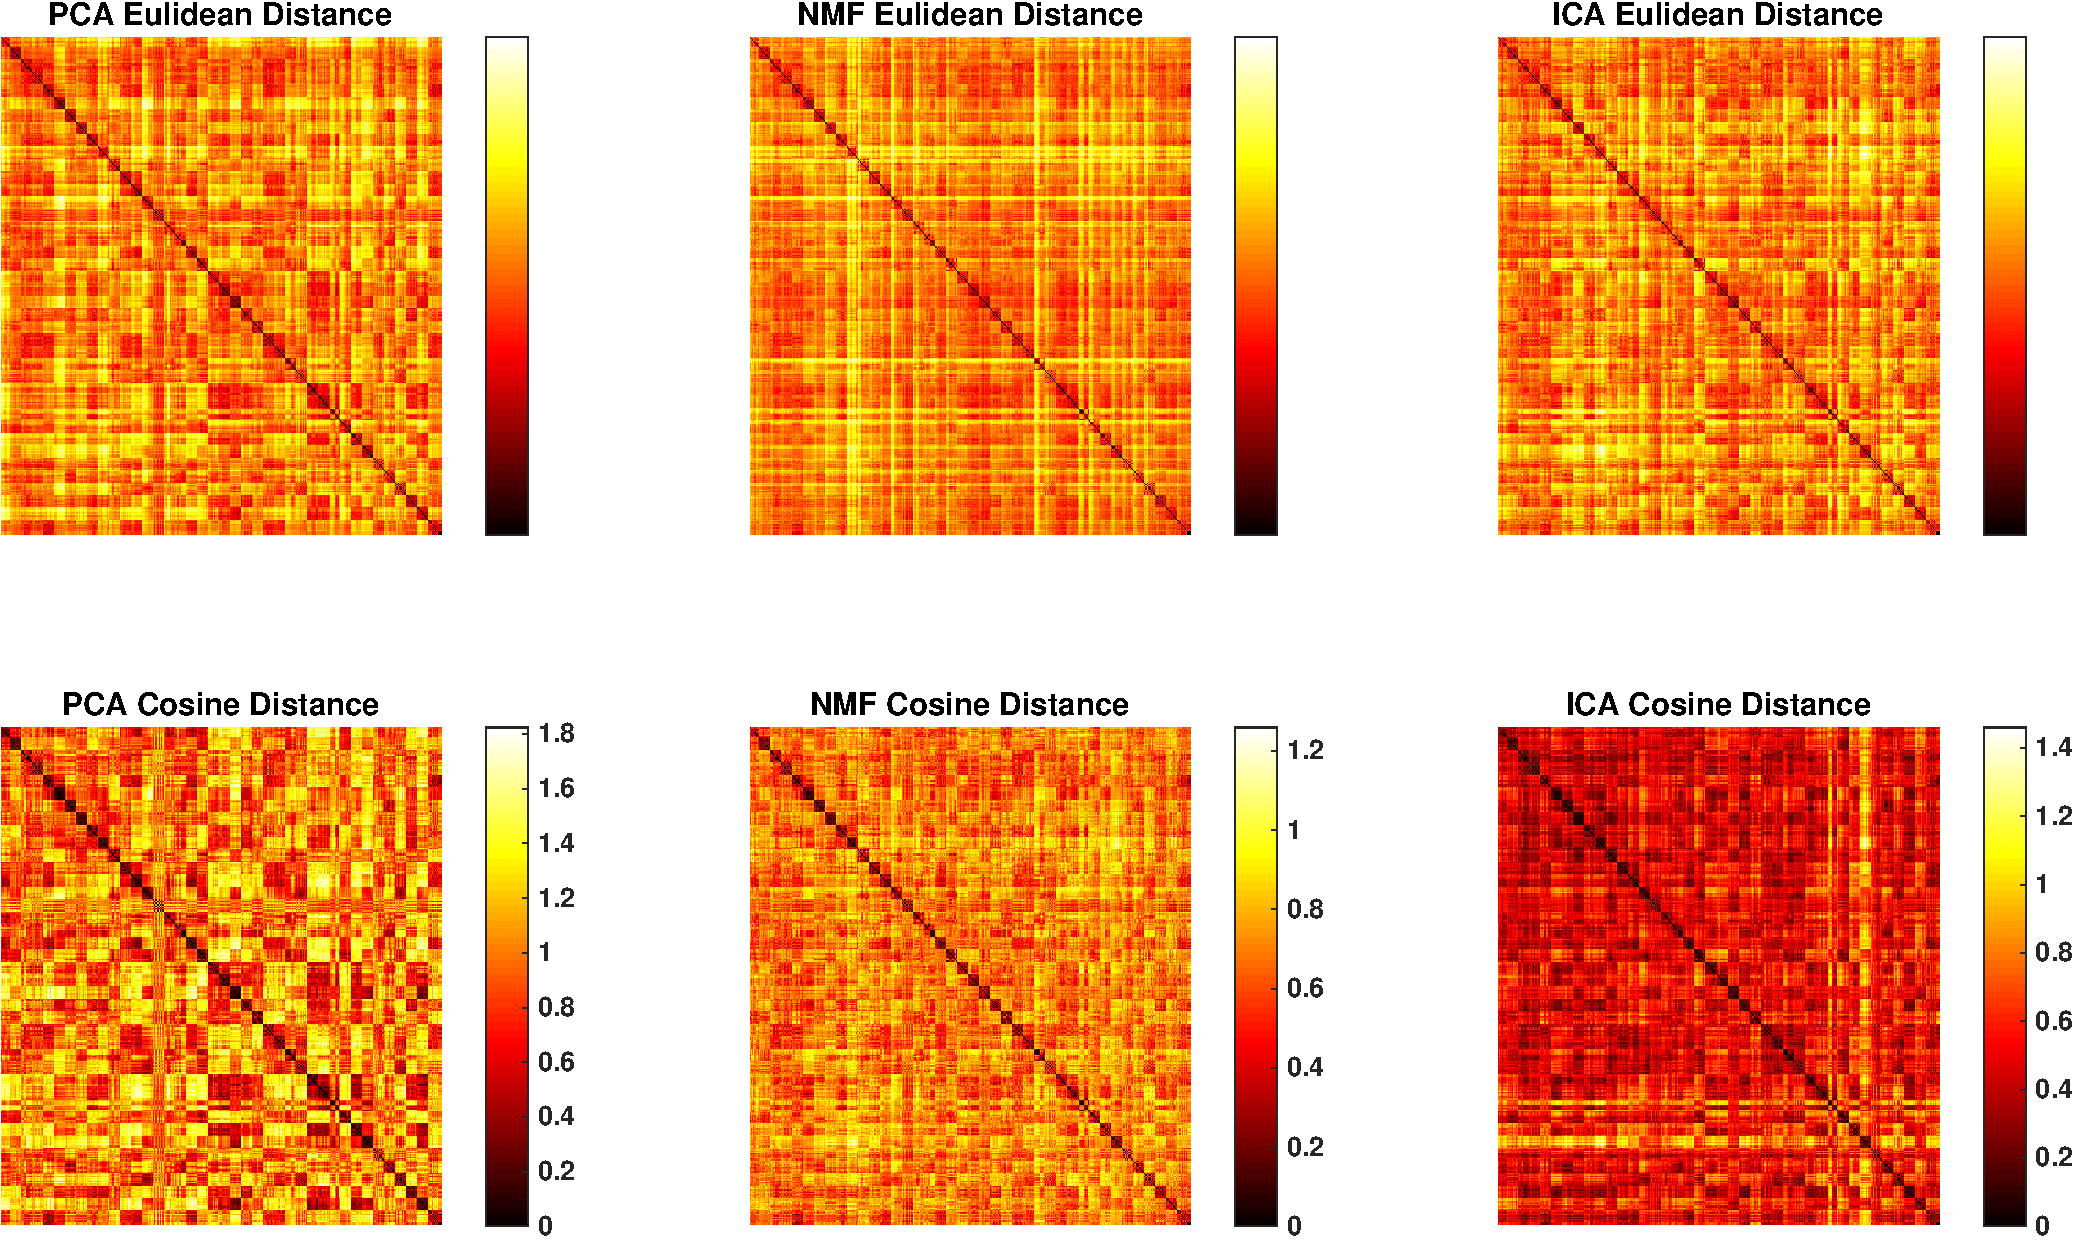
\includegraphics[width=1.1\textwidth]{Img/pni_dist} \captionof{figure}{PCA, NMF, ICA 投影权值的欧式距离和余弦距离}
}
\end{minipage}
\medskip
\end{center}

%
%\begin{center}
%\begin{minipage}[t]{\linewidth}
%%\label{fig:main}
%\center
%{
%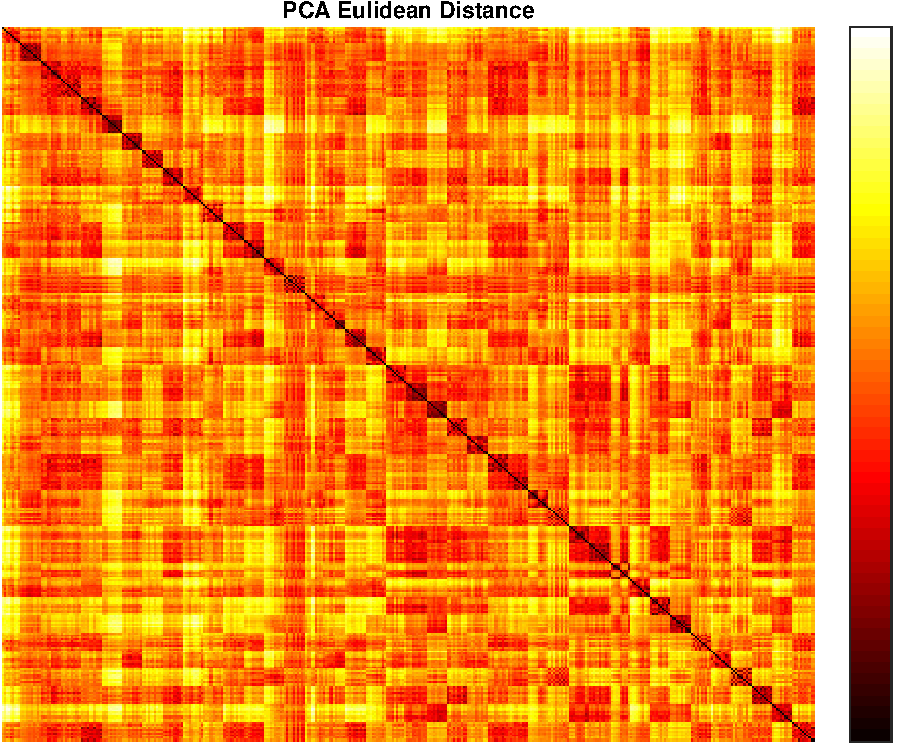
\includegraphics[width=\MyFactor\textwidth]{Img/pcaeu} \captionof{figure}{PCA Euclidean Distance}
%}
%\end{minipage}
%\medskip
%\end{center}
%
%\begin{center}
%\begin{minipage}[t]{\linewidth}
%%\label{fig:main}
%\center
%{
%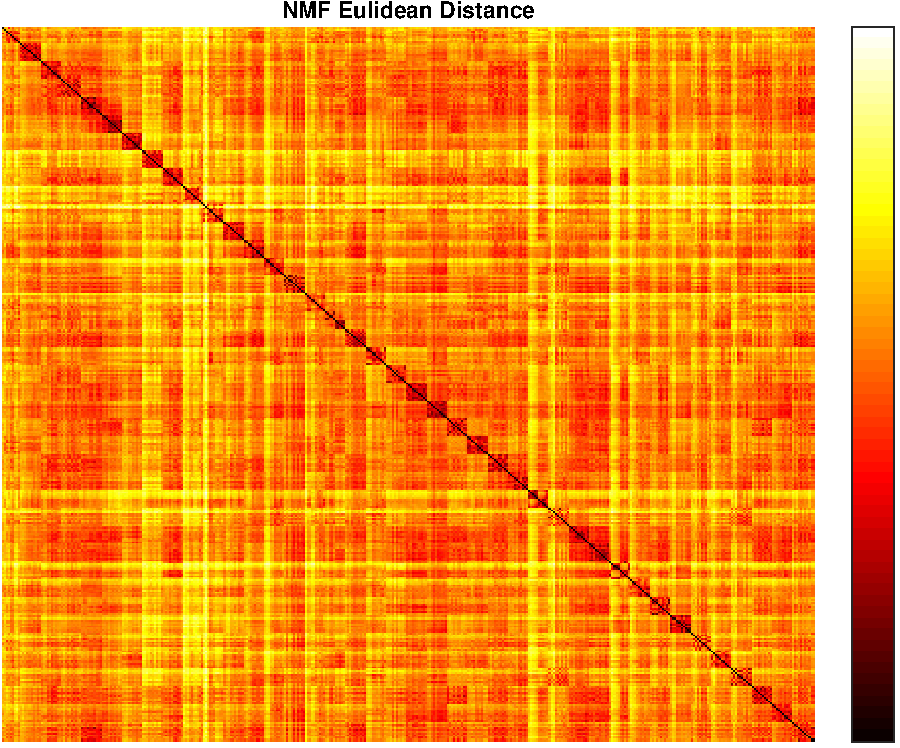
\includegraphics[width=\MyFactor\textwidth]{Img/nmfeu} \captionof{figure}{NMF Euclidean Distance}
%}
%\end{minipage}
%\medskip
%\end{center}
%
%\begin{center}
%\begin{minipage}[t]{\linewidth}
%%\label{fig:main}
%\center
%{
%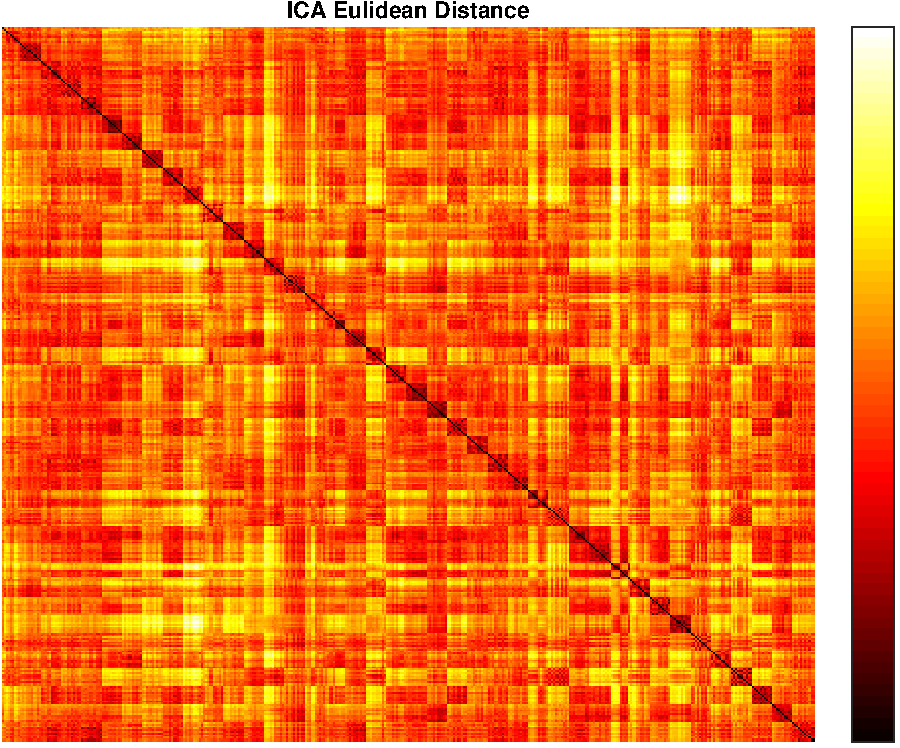
\includegraphics[width=\MyFactor\textwidth]{Img/icaeu} \captionof{figure}{ICA Euclidean Distance}
%}
%\end{minipage}
%\medskip
%\end{center}
%
%
%\begin{center}
%\begin{minipage}[t]{\linewidth}
%%\label{fig:main}
%\center
%{
%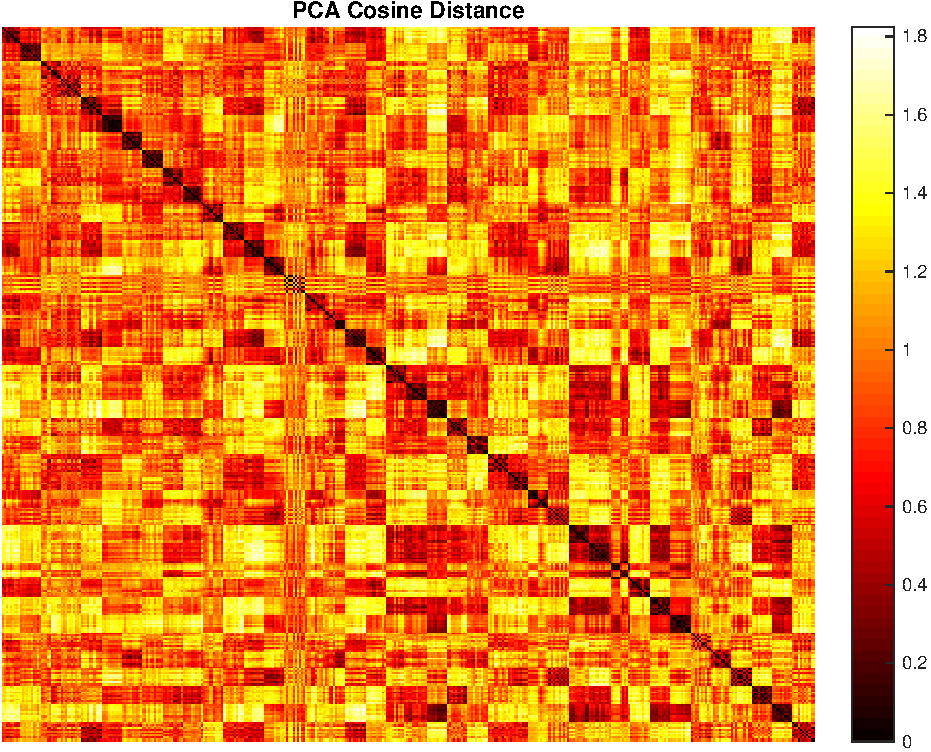
\includegraphics[width=\MyFactor\textwidth]{Img/pcacos} \captionof{figure}{PCA Cosine Distance}
%}
%\end{minipage}
%\medskip
%\end{center}
%
%\begin{center}
%\begin{minipage}[t]{\linewidth}
%%\label{fig:main}
%\center
%{
%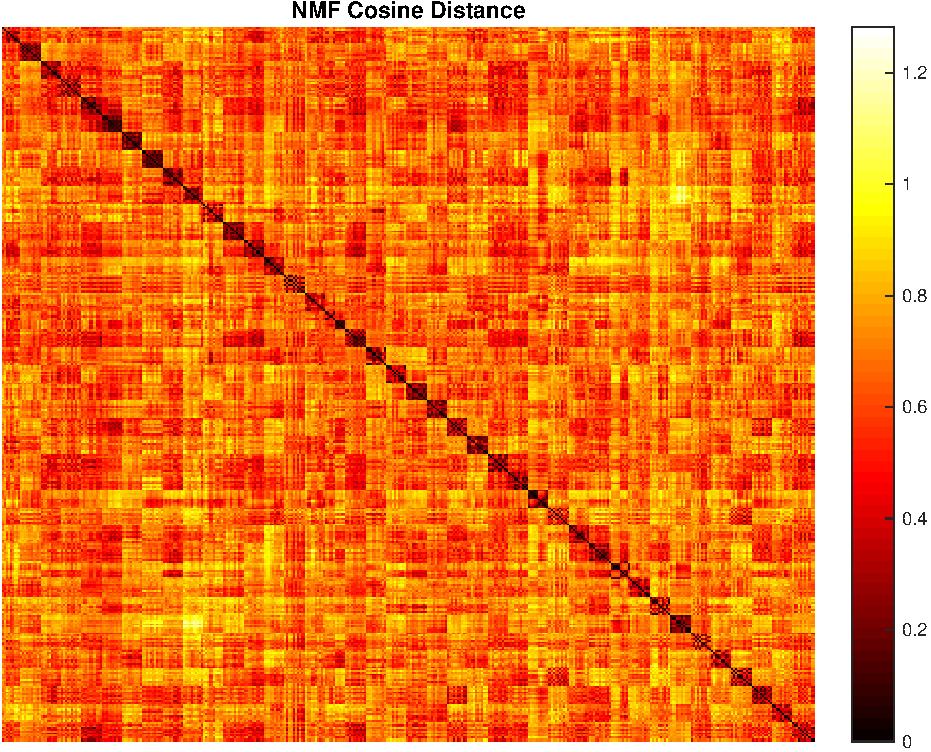
\includegraphics[width=\MyFactor\textwidth]{Img/nmfcos} \captionof{figure}{NMF Cosine Distance}
%}
%\end{minipage}
%\medskip
%\end{center}
%
%\begin{center}
%\begin{minipage}[t]{\linewidth}
%%\label{fig:main}
%\center
%{
%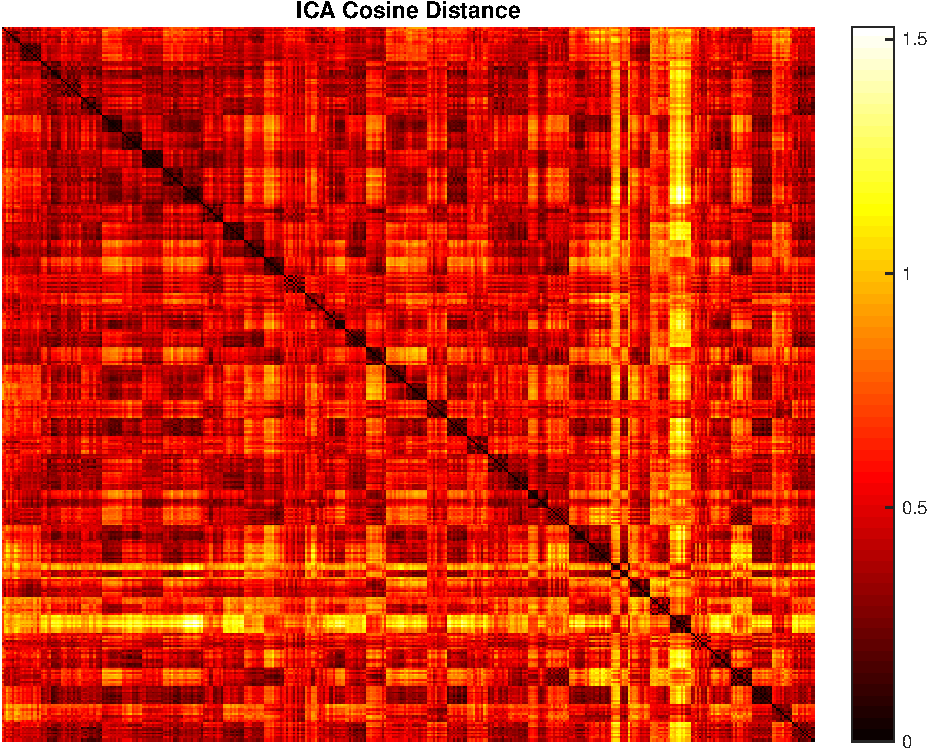
\includegraphics[width=\MyFactor\textwidth]{Img/icacos} \captionof{figure}{ICA Cosine Distance}
%}
%\end{minipage}
%\medskip
%\end{center}
%
\paragraph{结论}
\begin{itemize}
	\item 可见,上述6幅图片的对角线均存在着颜色约为黑色(取值为0),大小约为$10 \times 10$的方阵,说明这些算法都有能力将不同人,同一个人的照片区别开来.但是,这些图也有一些瑕疵,如,有些类间的距离比较小,有些说明类内距离比较大.
	\item 在两种比较尺度下,这三种算法的距离都有一定的区别,说明距离的度量和方法也有关系
\end{itemize}

\subsection{运行时间的比较}
\label{sec:pni_cal_time}
本章节分别创建[1, 11, 21, 31, 41, 51, 61, 71, 81, 91]维度的基底,并分别统计运算时间.
\paragraph{基底创建时间}
\begin{center}
\begin{minipage}[t]{\linewidth}
%\label{fig:main}
\center
{
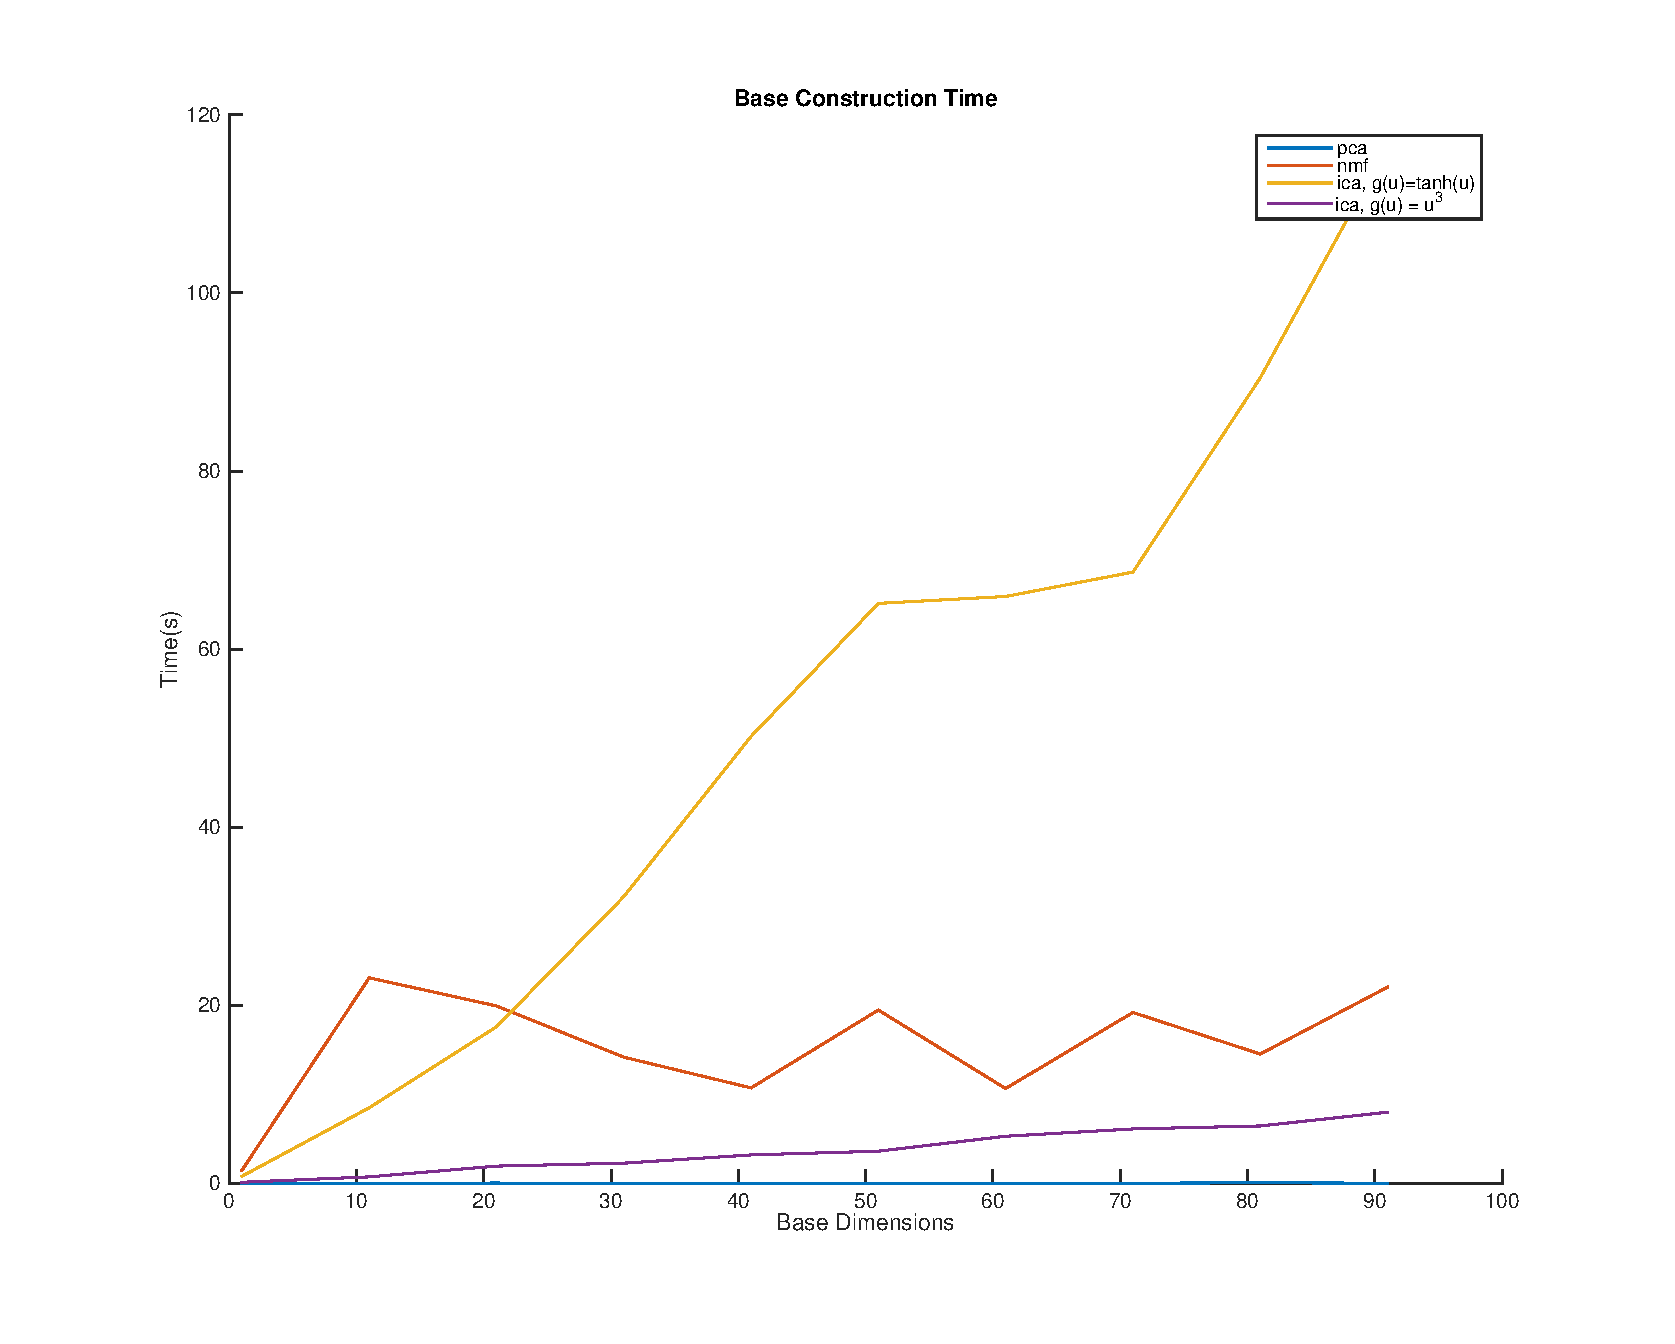
\includegraphics[width=\MyFactor\textwidth]{Img/pni_baseconstr} \captionof{figure}{基底创建时间 \\其中ICA分别用了两种不同的配置}
\label{fig:ica_base}
}
\end{minipage}
\medskip
\end{center}

\paragraph{基底投影时间}
\begin{center}
\begin{minipage}[t]{\linewidth}
%\label{fig:main}
\center
{
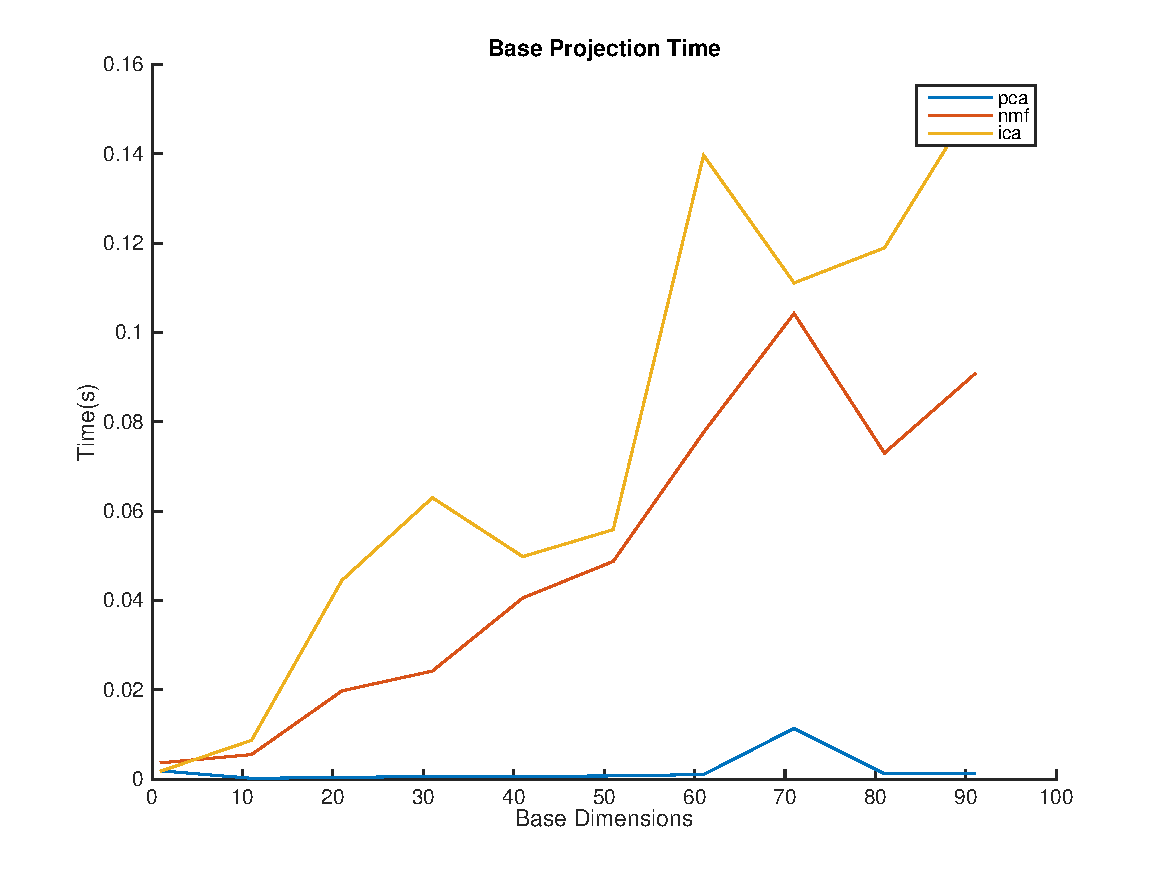
\includegraphics[width=\MyFactor\textwidth]{Img/pni_baseproj} \captionof{figure}{基底投影时间}
\label{fig:ica_base}
}
\end{minipage}
\medskip
\end{center}

\paragraph{结论}
\begin{itemize}
	\item PCA速度最快,并且优势明显,且对基底的数目不敏感。
	\item NMF, ICA运行速度比较慢,随着基底的增加运算量增大
	\item NMF, ICA迭代运算对初值敏感的特点,运行速度呈现波动
	\item 实际操作中,发现ICA的参数\ref{ica_g}对运行有较大影响
		$g(u)=tanh(a1*u)$时较慢,并且随样本数上升而增加计算量,$g(u) = u^3$时相比快很多,并且样本数的增加不敏感
	\item 与创建基底时间相比,投影时间小很多,所以可以离线计算基底,在线投影
	\item 同时,由于伪逆\textit{pinv()}的涉及,NMF,ICA运行需要时间,PCA求逆基本不需要时间
\end{itemize}



\subsection{重建与恢复}
\label{sec:pni_recon}
本小节是对PCA, NMF, ICA的恢复情况的比较.其过程是这样的,在\ref{sec:pni_cal_time}的基础上,分别选取5个样本来投影,并计算PSNR和MSE. 维度分别为[1, 11, 21, 31, 41, 51, 61, 71, 81, 91].
\begin{enumerate}
	\item 第一张样本是ORL数据库中已有的一张图片,该图片参与了基底运算
	\item 第二张样本是ORL数据库中已有的一张图片,该图片没有参与基底运算
	\item 第三张样本是一张普通的人脸图片
	\item 第四张是上一张图片去除背景的部分(使用了\textit{Viola-Jones algorithm}来识别人脸)
	\item 第五张样本是一个非人脸图片
\end{enumerate}

	\begin{center}
	\begin{minipage}[t]{\linewidth}
	\center
	{
	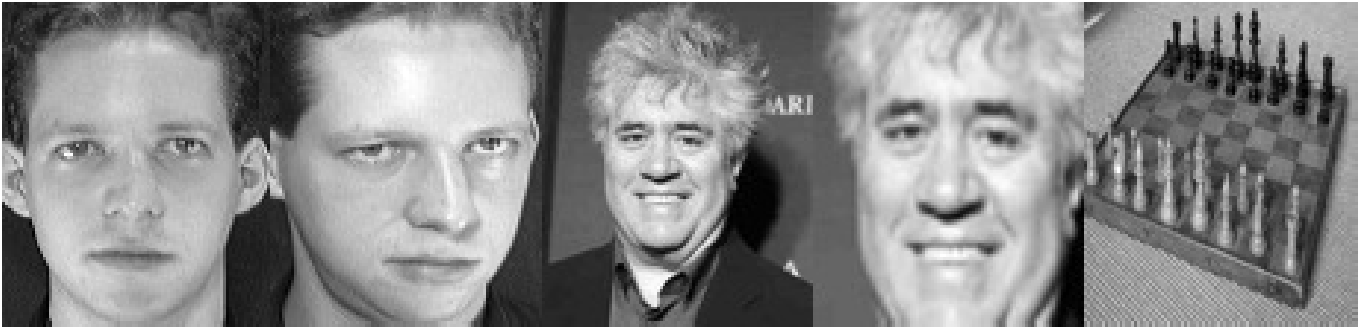
\includegraphics[width=\MyFactor\textwidth]{Img/pni_recon} \captionof{figure}{重构输入样本示意}
	}
	\end{minipage}
	\medskip
	\end{center}

	\paragraph{重建结果}
\begin{center}
\begin{minipage}[t]{\linewidth}
\center
{
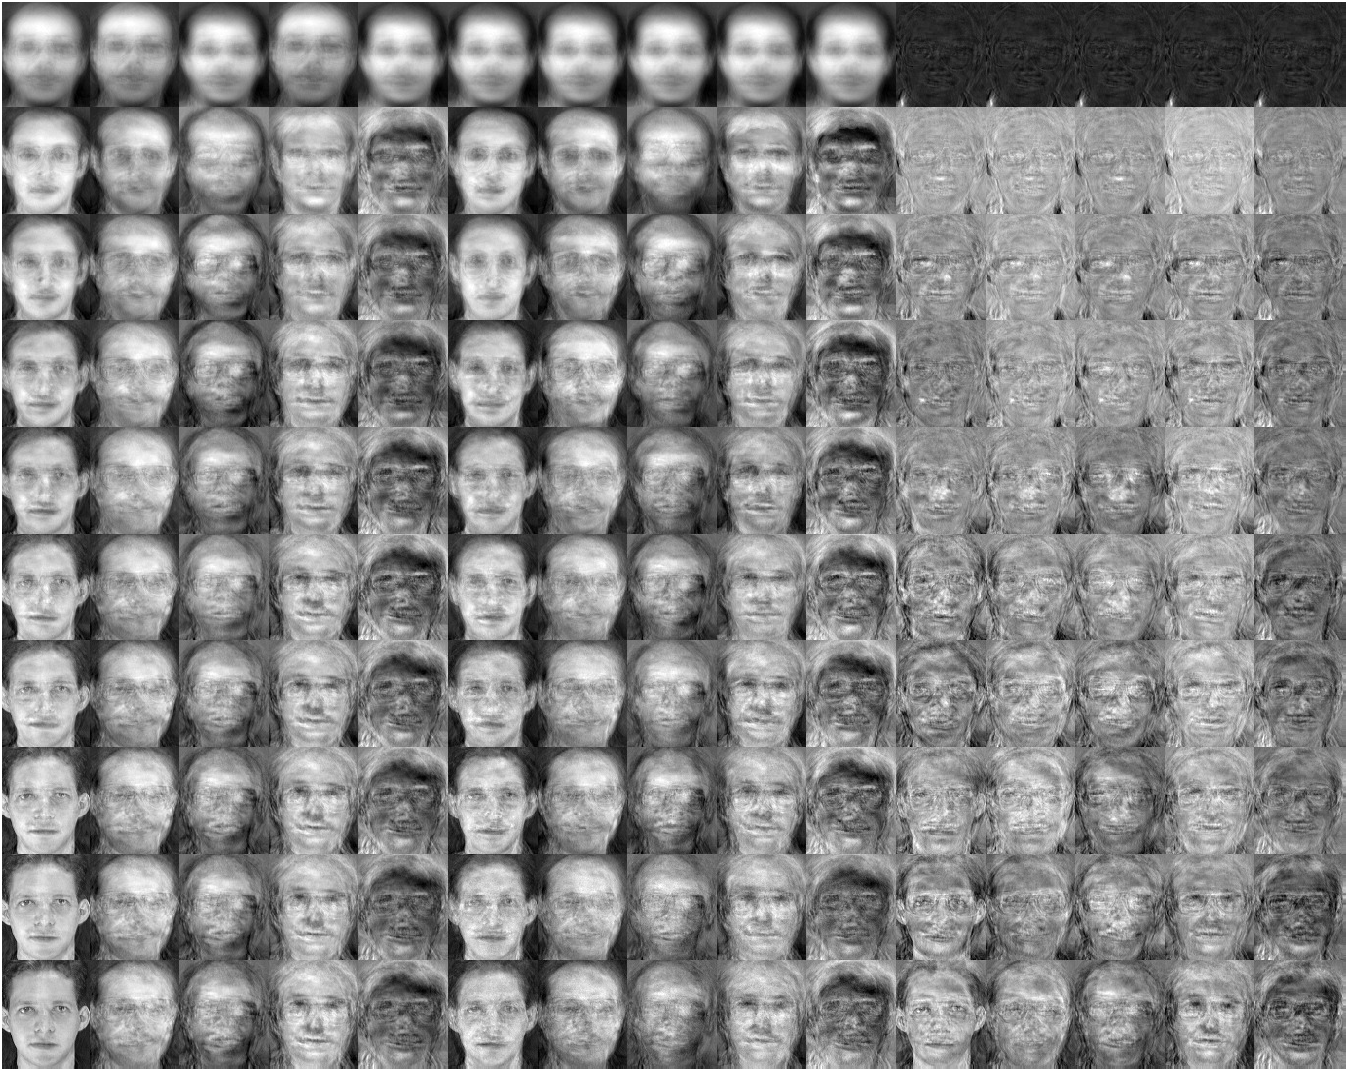
\includegraphics[width=\textwidth]{Img/pni_recon_re} \captionof{figure}{测试图像的投影\\横轴:左5:PCA, 中5: NMF, 右5: ICA, 纵轴: 维度依次增加}
	\label{fig:pni_recon_re}
}
\end{minipage}
\medskip
\end{center}
\paragraph{MSE}
MSE的公式为\begin{equation}
		MSE = \Sigma_{i=1}^m\Sigma_{j=1}^n(Y(i,j) - X(i,j))^2	\end{equation}
	
	\begin{enumerate}
	\item m,n 是图片的尺寸
	\item X,Y 分别是恢复及重建的图片
\end{enumerate}

\begin{center}
\begin{minipage}[t]{\linewidth}
\center
{
		\captionsetup{justification=centering}
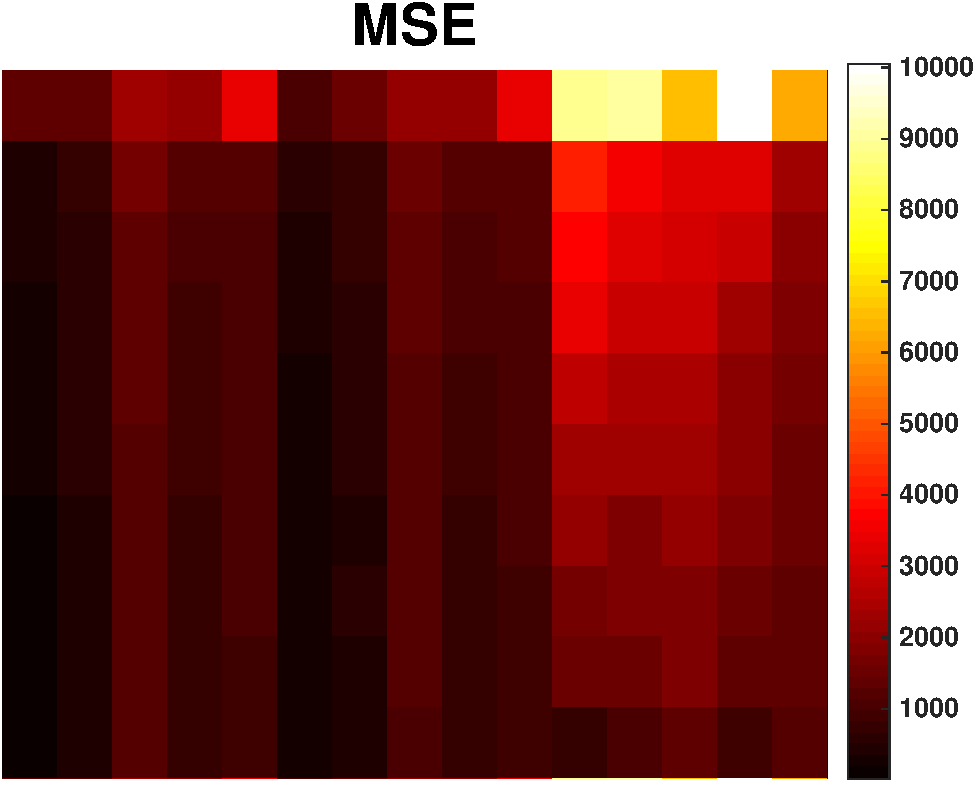
\includegraphics[width=\textwidth]{Img/pni_rec_mse} \captionof{figure}{与\ref{fig:pni_recon_re}对应的MSE \\横轴:左5:PCA, 中5: NMF, 右5: ICA, 纵轴: 维度依次增加}
\label{fig:ica_base}
}
\end{minipage}
\medskip
\end{center}

\paragraph{结论}
\begin{itemize}
	\item 维数越高恢复结果越好
	\item 基于特征提取的人脸恢复图像恢复结果只能是和基底相关的图像.测试5的棋盘和恢复结果差别就比较大
	\item 对于参加特征提取的图像,恢复效果比较好,但对于大部分样本恢复效果并不好
	\item 维度的增加只意味着细节的增加,如PCA在30维的结果和100维的结果就已经很相近了
	\item 就恢复效果来说,PCA应该最适合开发,PCA不仅可以有\textit{eigenvalues}给出一个恢复效果的估计,同时计算也比较快,恢复效果也不差.
	\item 这种压缩方法其实并不合适,更好的方法应该是采用分块的方式,由于压缩比率过大,才使得恢复效果这么差的
\end{itemize}


\subsection{结合\textit{One-Against-All} SVM的分类实验}
\paragraph{识别结果} 当全局特征提取后,自然地,对这些样本本项目尝试了使用SVM的分类识别的测试.其实验过程:
	\begin{enumerate}
		\item 采用\textit{Cross Validation Hold Off}的方法,改变学习样本范围从10\%到90\%.选择样本时,每个人的样本均被随机同比例地分割
		\item 每个学习样本又同时对应了不同的基底长度
		\item 将学习,测试样本予以投影,并取得对应权值
		\item 具体测试是指对ORL数据库40个人,通过学习样本的标签来推测测试样本的标签
	\end{enumerate}
	
	
	经过上述的测试过程后,以下是实验的结果,其中
	\begin{enumerate}
		\item 识别率由z轴表示
		\item 从$5-100$变化的轴表示了基底的数量
		\item 从$1-9$变化的轴表示了学习的样本比例,以10\%为单位
	\end{enumerate}
	
	\begin{center}
	\begin{minipage}[t]{\linewidth}
	%\label{fig:main}
	\center
	{
	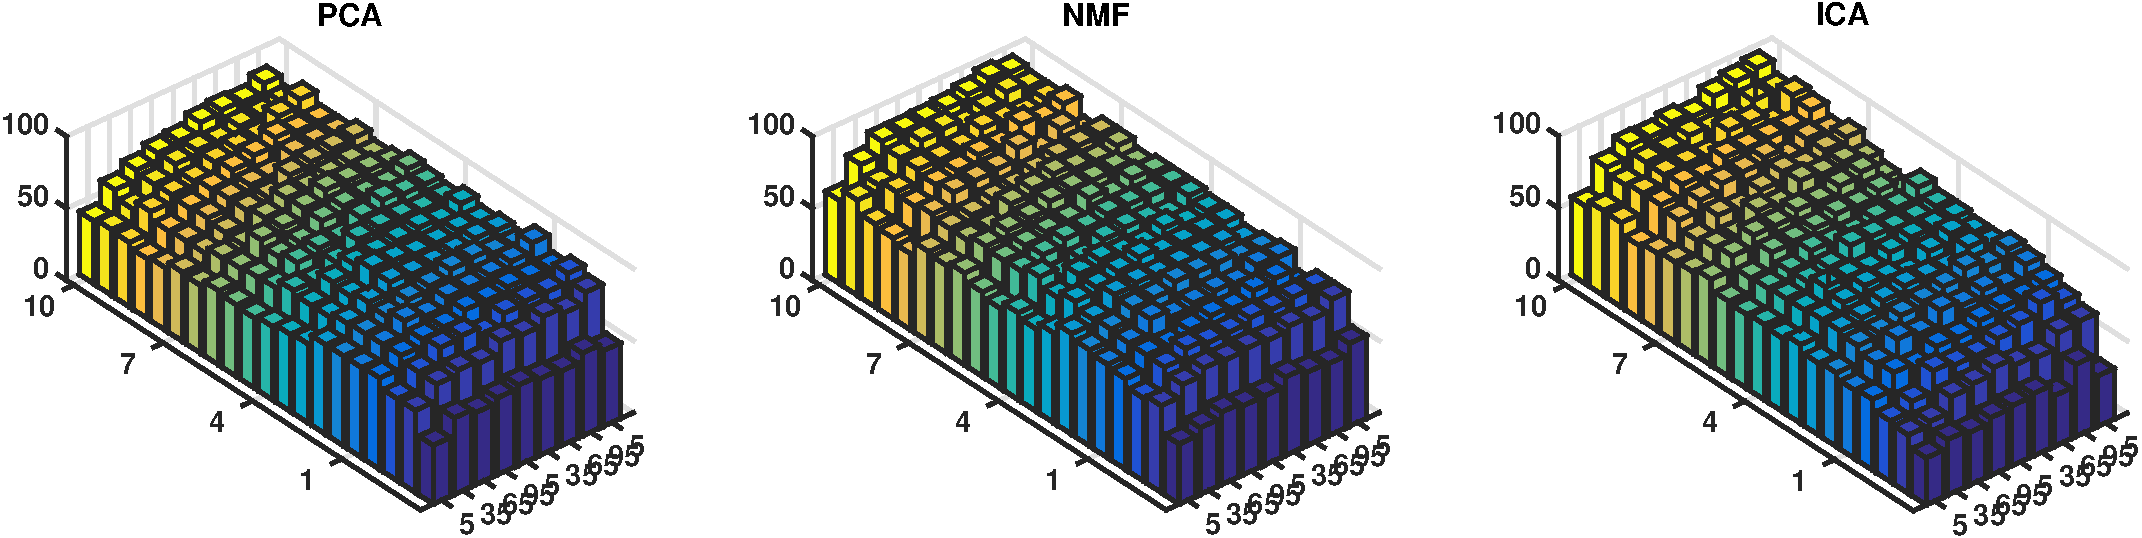
\includegraphics[width=\textwidth]{Img/svm_pni} \captionof{figure}{PCA, NMF, ICA结合SVM的分类实验}
	}
	\end{minipage}
	\medskip
	\end{center}

	
	下图将三张图片画到了一起,	
	\begin{center}
	\begin{minipage}[t]{\linewidth}
	\center
	{
	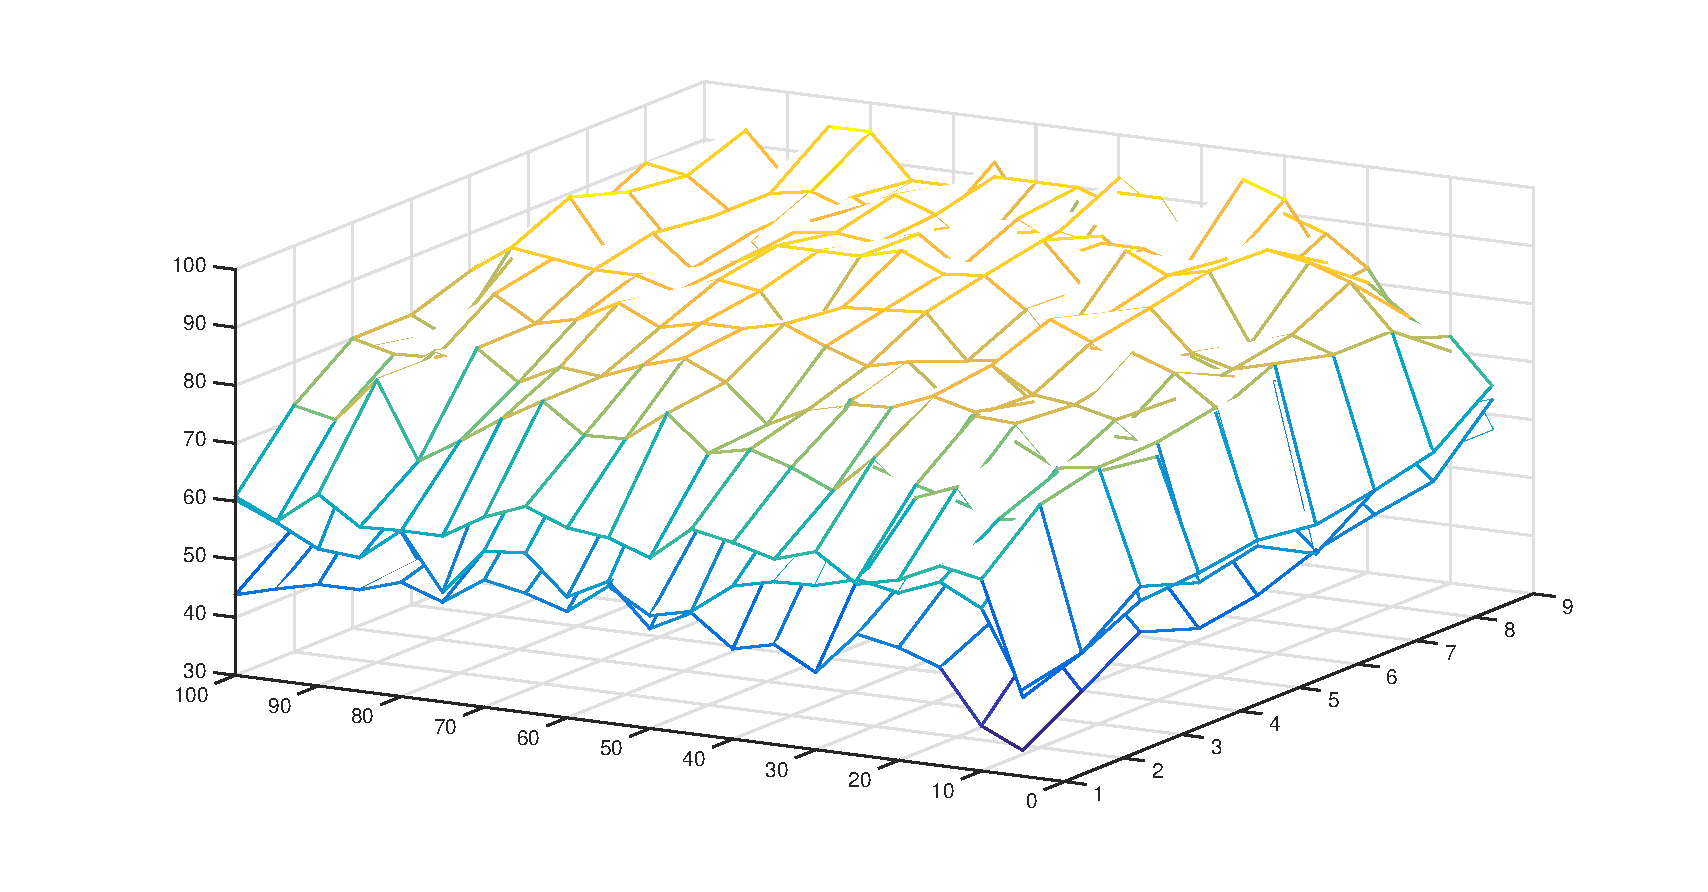
\includegraphics[width=\textwidth]{Img/svm_pcanmfica} 
	
	\captionof{figure}{SVM结合PCA,NMF,ICA识别实验}
	}
	\end{minipage}
	\medskip
	\end{center}
	发现三种基底结合相同的SVM的识别率发生了有了一些交叉.其中ICA的表现比较差,NMF在大部分区域表现比较好,而PCA在较短的向量部分表现比较好.
	
	\paragraph{对识别结果的过滤} 同时,还对以上的识别结果进行了过滤,来更清楚的表示识别率和样本数,基底数的关系
	
		\begin{center}
	\begin{minipage}[t]{\linewidth}
	\center
	{
	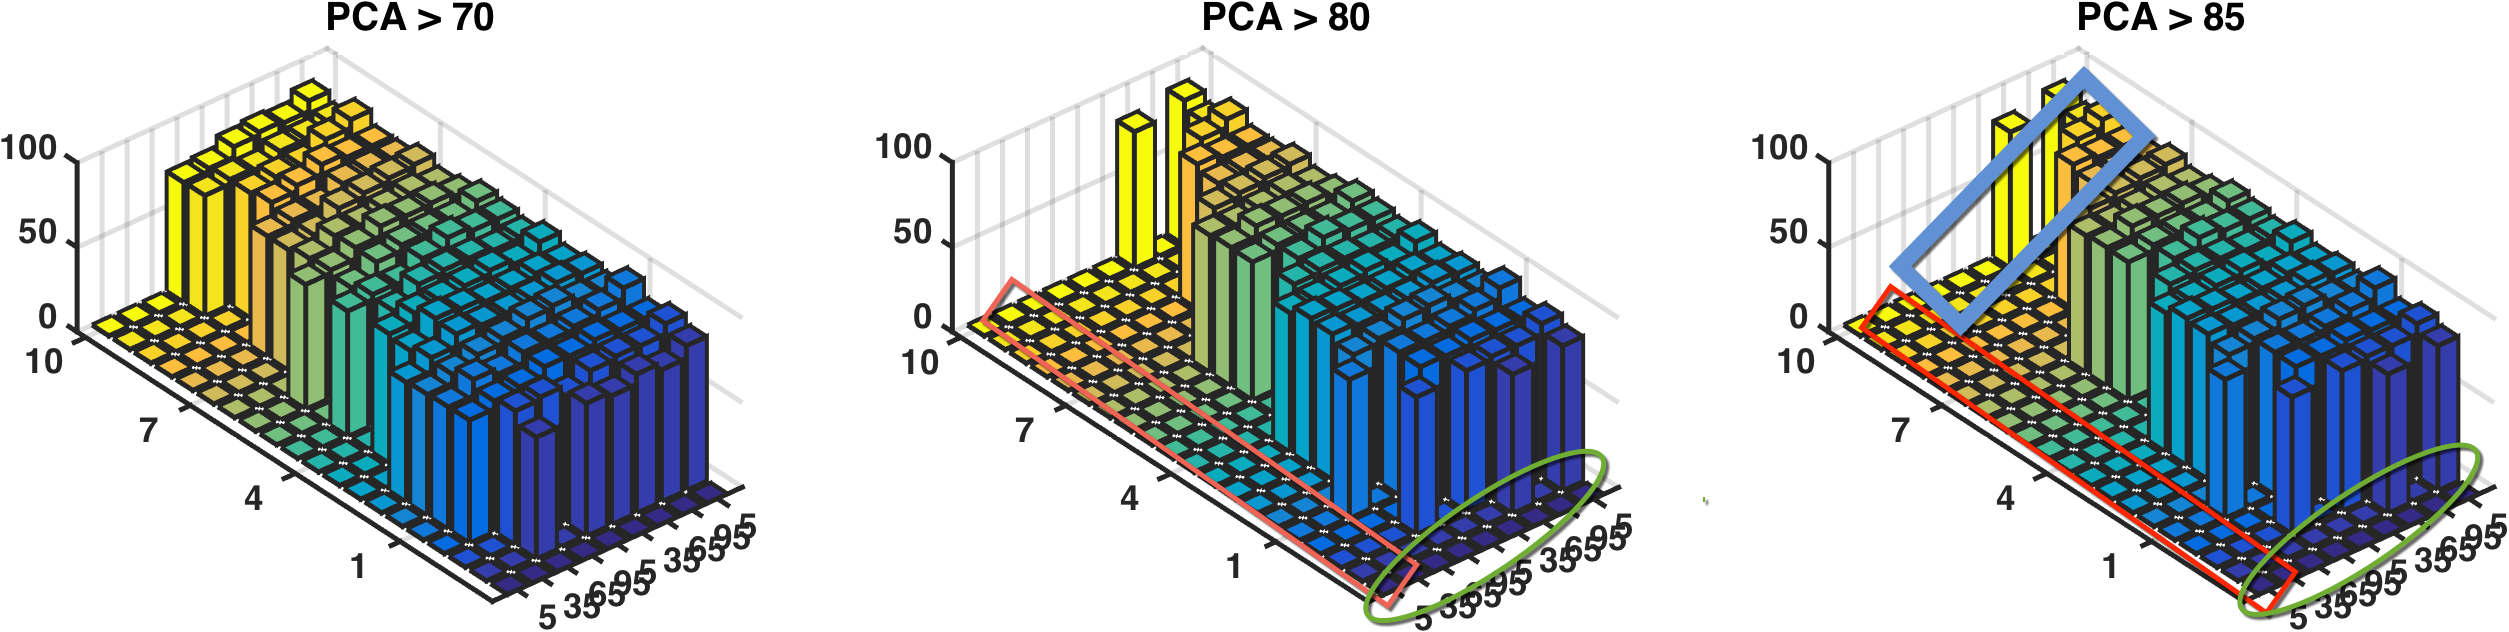
\includegraphics[width=\textwidth]{Img/svm_pcafilter} 
		\captionsetup{justification=centering}\captionof{figure}{SVM结合PCA不同识别率\\绿色:学习样本过少,红色:维数过低,蓝色:维数过高}
	}
	\end{minipage}
	\medskip
	\end{center}
	
	\paragraph{结论}
	\begin{itemize}
	\item 特征向量越多,在充分学习的情况下,其表现会越好,但这种优势并不明显,通常,特征向量$15-30$长度就足够满足需求了。
	\item 更多的特征向量会要求更多的学习样本,当映射使用了很多特征向量时,会增加对样本的需求,并降低其最终的识别率。
	\end{itemize}	
	
	\paragraph{在其他的空间上实现识别} 以上NMF, ICA的识别率不如PCA的好,这也许是空间的分布的缘故.于是,我想到了使用DCT等算法对空间进行转化,并在频率空间上进行识别.(由于NMF是非负分解,而DCT转化后的空间像素值可以为负,所以没有在NMF空间上使用DCT方法) \newline
	
	以下是普通ORL样本和DCT滤波后的ORL样本:
	
	\begin{center}
	\begin{minipage}[t]{\linewidth}
	%\label{fig:main}
	\center
	{
	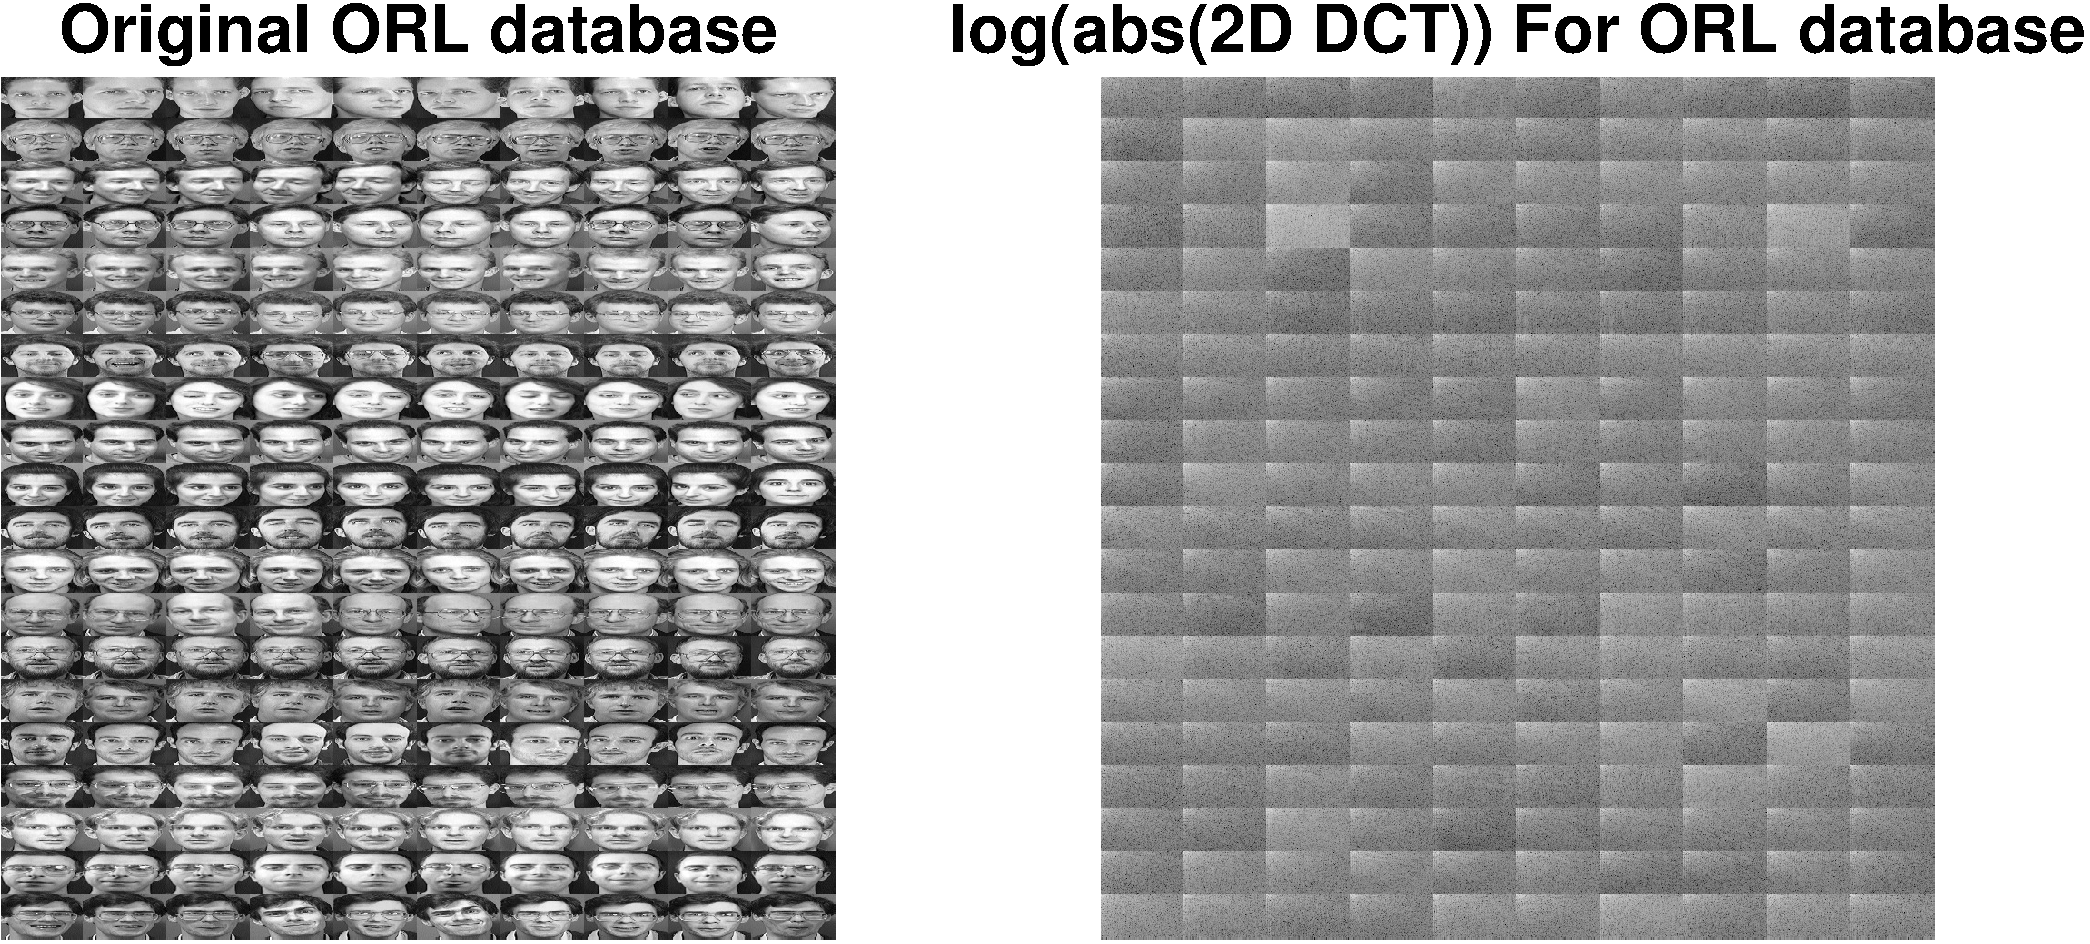
\includegraphics[width=\textwidth]{Img/dct_demo} \captionof{figure}{DCT演示(仅前20个人的数据)}
	}
	\end{minipage}
	\medskip
	\end{center}

	以下是数据改换成DCT数据后的PCA降维后结合SVM分类的结果.
	\begin{center}
	\begin{minipage}[t]{\linewidth}
	%\label{fig:main}
	\center
	{
	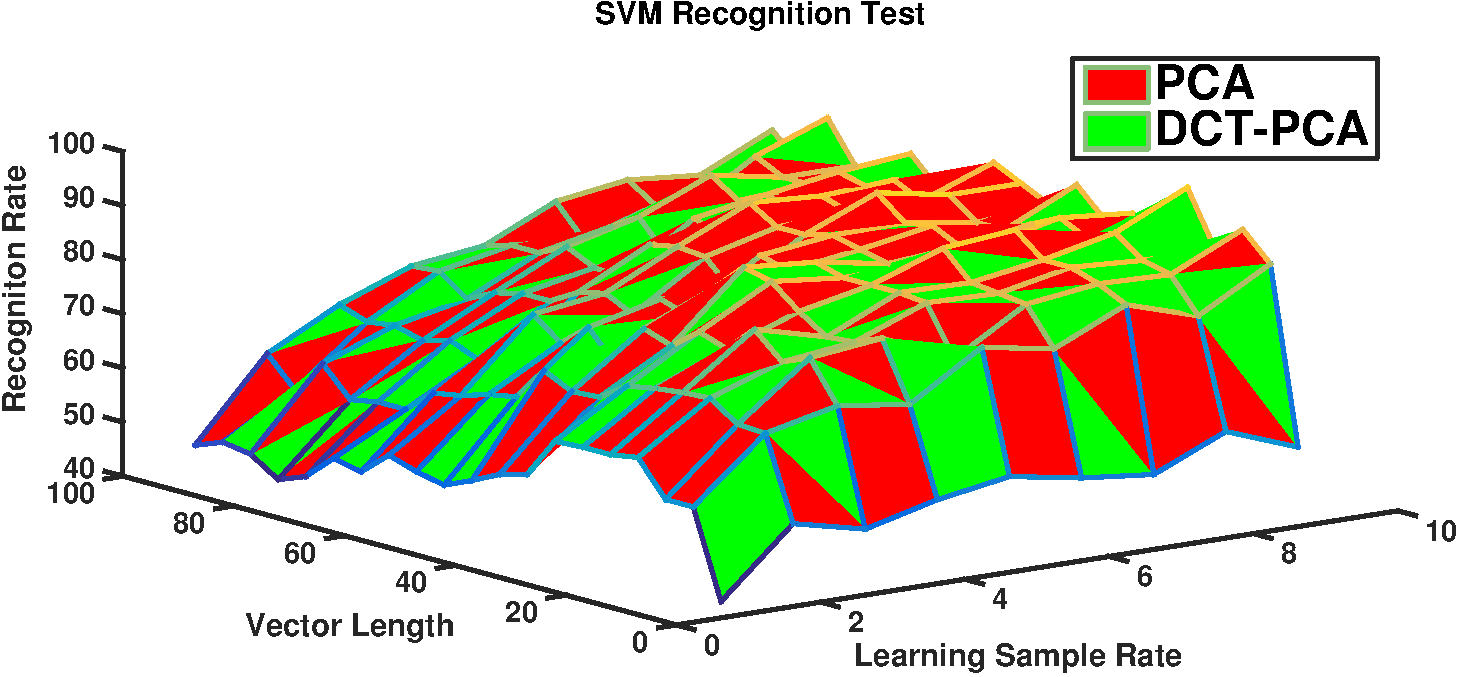
\includegraphics[width=\textwidth]{Img/svm_pca_dct} \captionof{figure}{PCA, DCT-PCA结合SVM实验}
	}
	\end{minipage}
	\medskip
	\end{center}
	PCA与DCT-PCA完全重合,说明DCT处理后对其性能没有提升.
	
	\begin{center}
	\begin{minipage}[t]{\linewidth}
	%\label{fig:main}
	\center
	{
	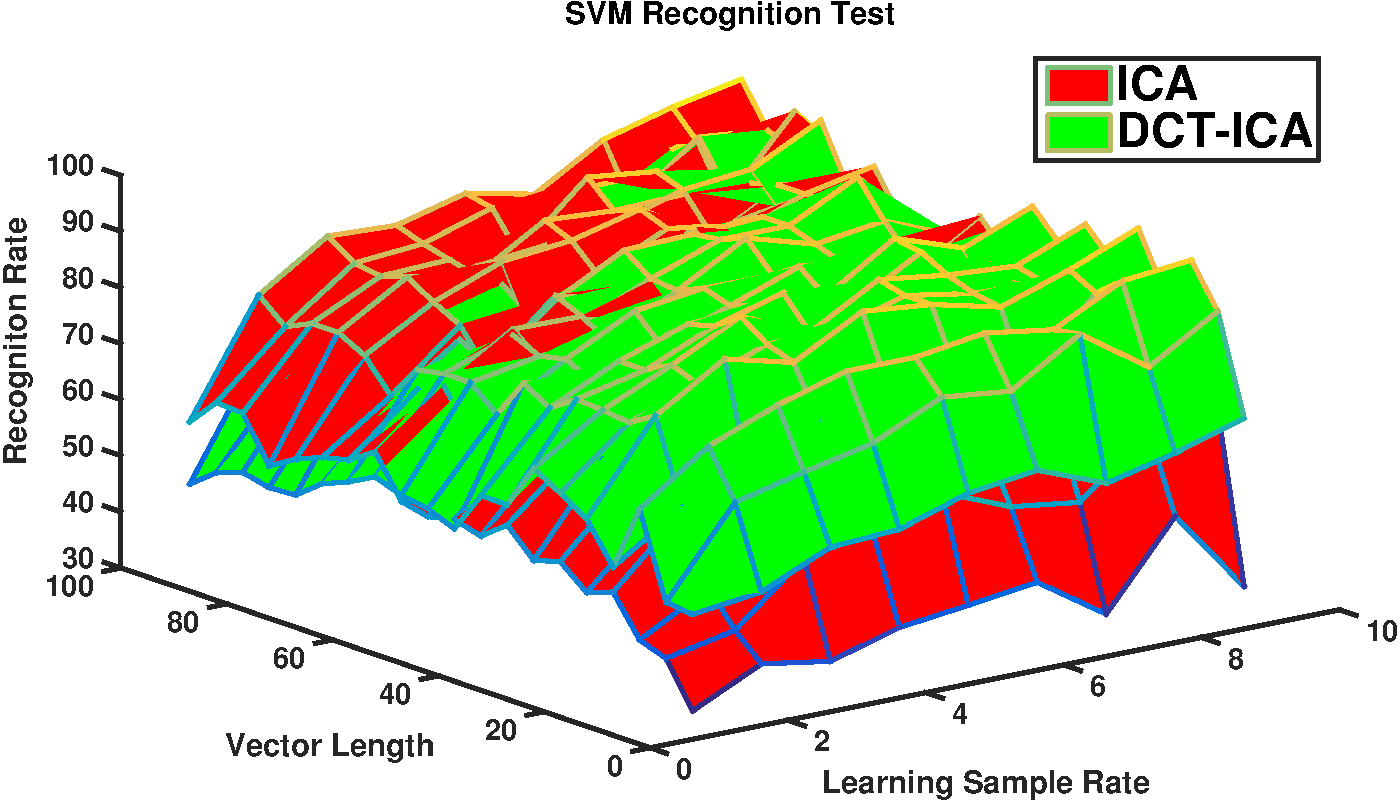
\includegraphics[width=\textwidth]{Img/svm_ica_dct} \captionof{figure}{ICA, DCT-ICA结合SVM实验}
	}
	\end{minipage}
	\medskip
	\end{center}
	DCT处理后,显著提升了ICA的性能,使得ICA在特征向量较短的情况下能取得更加好的成功识别率.
	
	\paragraph{结论}
	\begin{itemize}
		\item 确实可以提高ICA的识别率.所以处理的空间对样本来说也比较重要.
		\item 识别到一定成功率后,基于全局的方法出现了瓶颈.参考下面列出的易于出错的样本,发现这主要由于有些样本比较相似导致的
	\end{itemize}
	\paragraph{识别错例}
	以下错例取自学习样本为90\%的NMF结合PCA的运行程序,共测试了40次,识别率为85\%,下面是对运行结果中出错的6个例子的分析:
	\begin{center}
	\begin{minipage}[t]{\linewidth}
	%\label{fig:main}
	\center
	{
	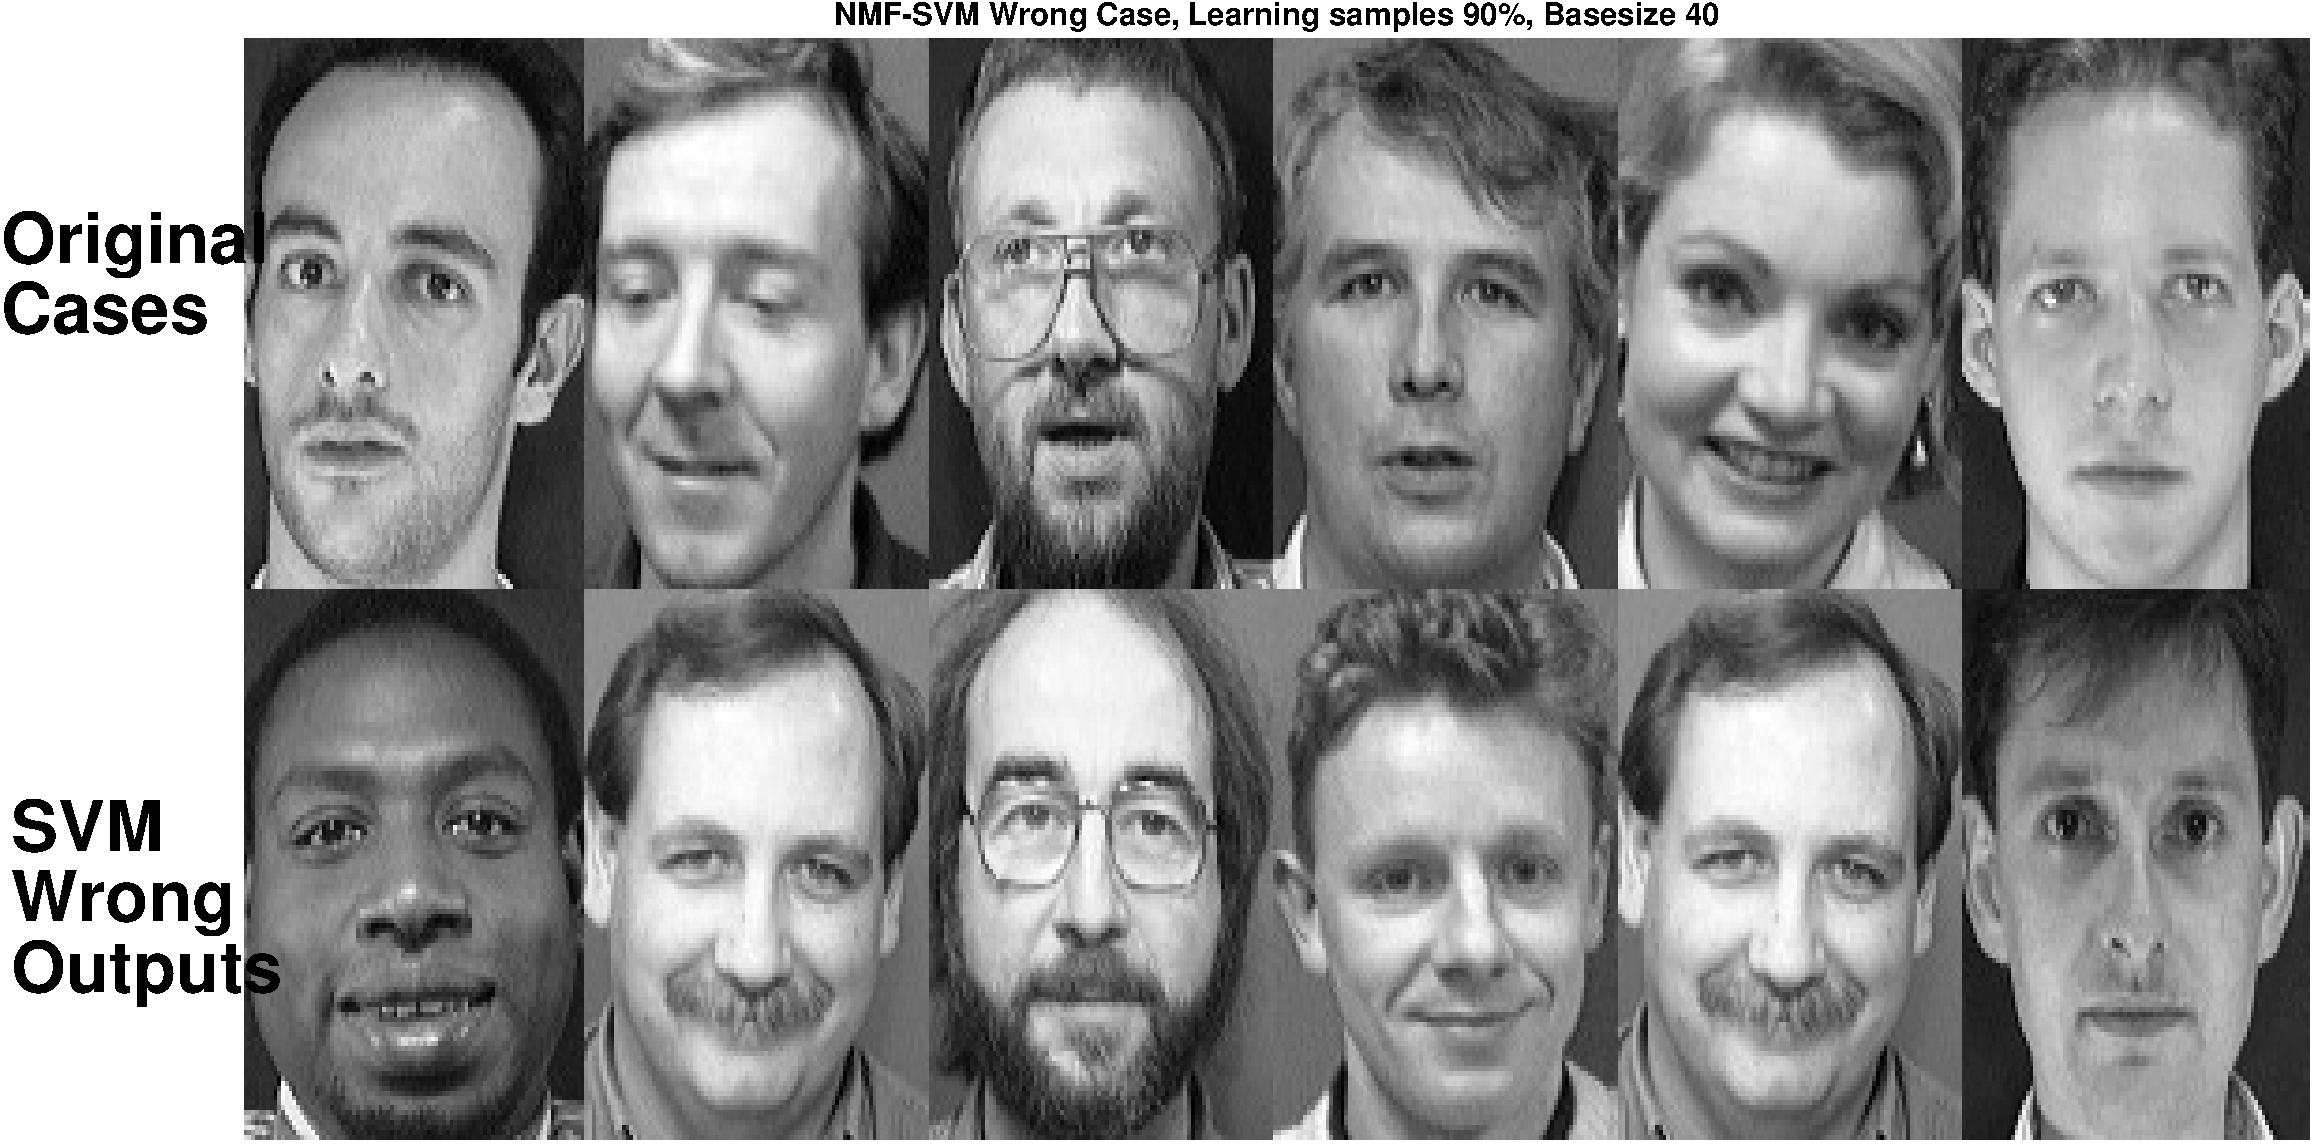
\includegraphics[width=\textwidth]{Img/svm_wrong} \captionof{figure}{上:输入的样本,下:预测的样本}
	}
	\end{minipage}
	\medskip
	\end{center}
	以下是对应出错的例子的标签:
	\begin{center}
	\captionof{table}{SVM出错的例子的标签}\begin{tabular}{|l|l|l|l|l|l|l|}
\hline
原本标签&16&3&14&15&35&1\\\hline
误测标签&22&25&28&21&25&24\\\hline
\end{tabular}
\end{center}

	
	从上面的示意图中可以看到,有些样本是比较相似的,而由于基于全局的特征提取方法无法做到精细的比较,所以出错了.如,倒数第一,二,三个样本人脸的角度就和预测的人脸角度比较一样.再如,第三个人脸的胡子的特征就和预测的人脸比较一样.
	
\paragraph{Confusion Matrix}

Confusion Matrix是表征分类情况的图像,以下是某次SVM运行的结果,采用了5-fold Validation.综合成功率94\%.特征提取算法是PCA.

	\begin{center}
	\begin{minipage}[t]{\linewidth}
	%\label{fig:main}
	\center
	{
	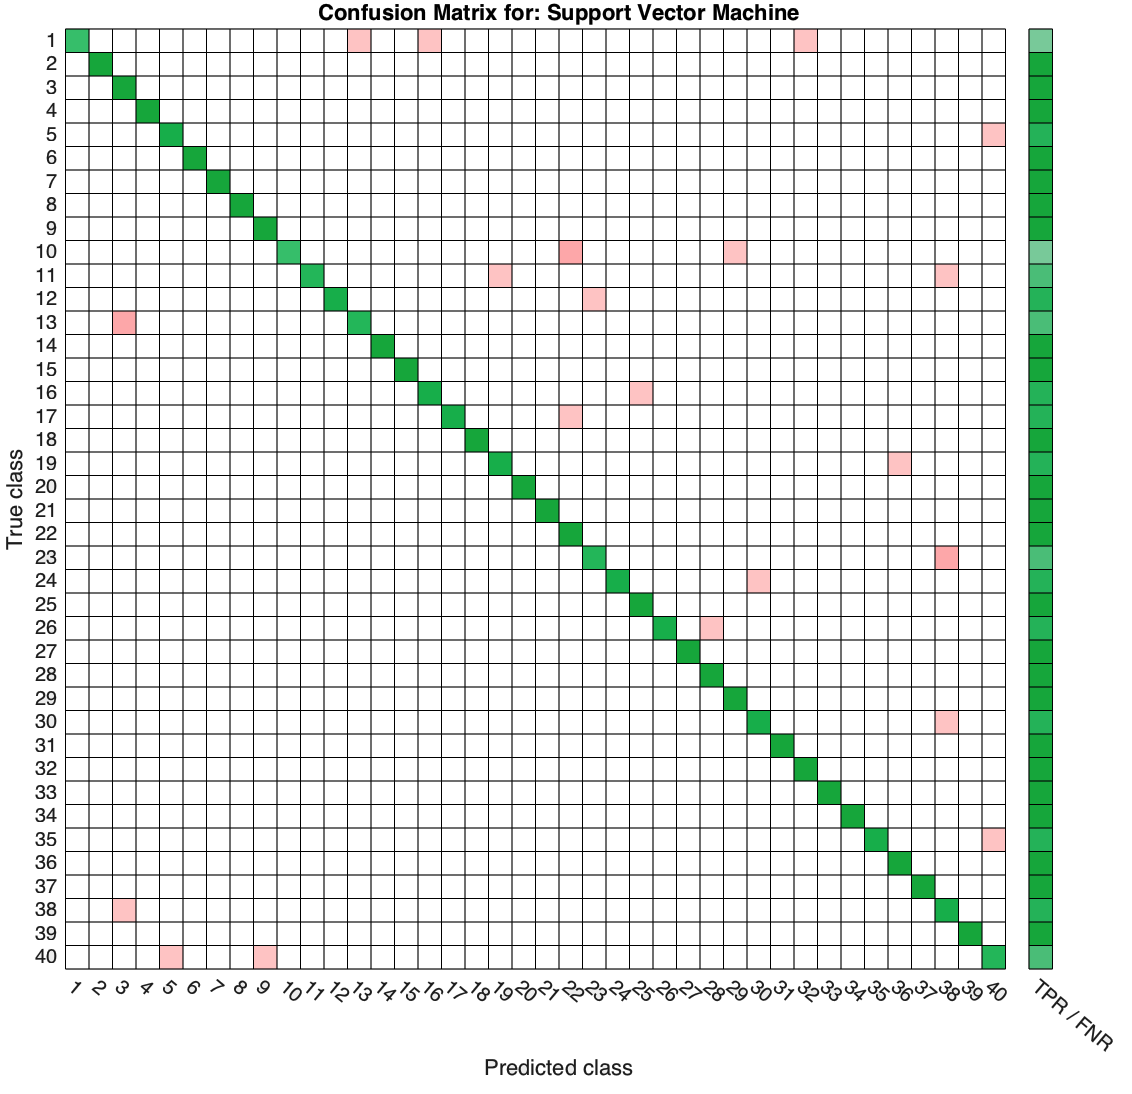
\includegraphics[width=\textwidth]{Img/svm_confuse} \captionof{figure}{Confusion Matrix}
	}
	\end{minipage}
	\medskip
	\end{center}
	可以发现,大部分结果是正确的,同时,也发现了一定的对称性,说明有些样本易于混淆,比如,SVM分类40号样本时误认为部分是5号样本的,当分类5号样本时,由误认了部分样本是40号的.说明全局的特征提取算法无法分析细节,所以只能给出大概的估计.
	

\subsection{结合多种分类模型的分类实验}

上一节详细使用了SVM作为分类机,本节将遍历分类算法,来综合测试.具体过程如下:
	\begin{enumerate}
		\item PCA, NMF, ICA均从ORL数据库40人的前3张图片计算出该组数据库的长度为64位的基底.
		\item ORL数据库每个样本参加基底运算的3张图片和没有参加的7张图片全部被上一步的运算投影成为长度为64的坐标
		\item 结合原有的标签,采用\textit{3-folds Cross-Validation}的方法,进行分类测试,并记录准确率
	\end{enumerate}




下图是运行过程的截图:
	
		\begin{center}
	\begin{minipage}[t]{\linewidth}
	%\label{fig:main}
	\center
	{
	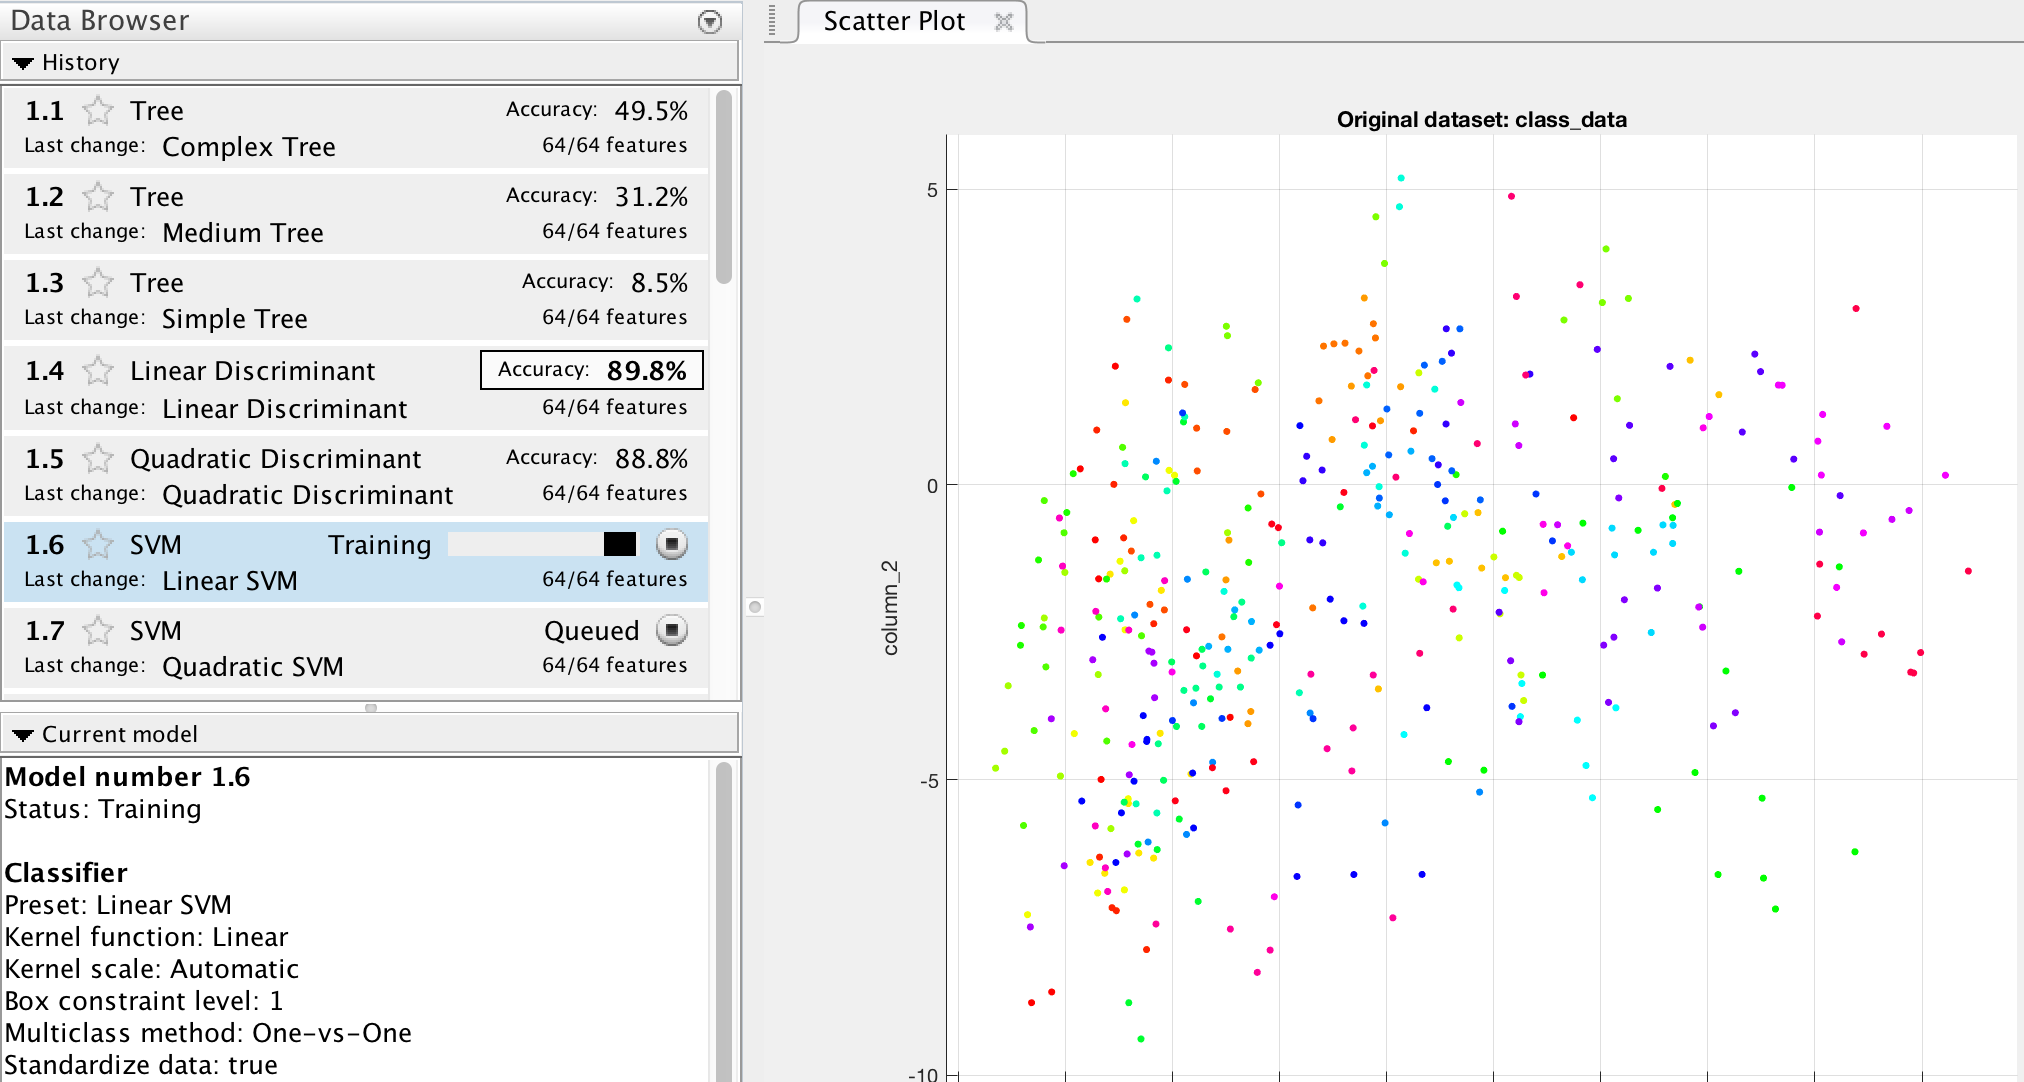
\includegraphics[width=\textwidth]{Img/class_training} \captionof{figure}{使用\textit{Matlab Classification Learner}进行分类机遍历}
	}
	\end{minipage}
	\medskip
	\end{center}

	
		\newpage
\paragraph{本项目研究的特征提取算法}
\begin{center}
\captionof{table}{PCA,NMF,ICA, DCT PCA, DCT ICA结合不同分类机的分类效果}
\label{table: classifiers}
\begin{tabular}{|l|l|l|l|l|l|l|}
\hline
&Method&PCA&NMF&ICA& DCT PCA & DCT ICA\\\hline
1&Complex Tree &56.2&52.5&52.2&57.5&63.5\\\hline
2&Medium Tree & 34.2&32&28&32.2&35.5\\\hline
3&Simple Tree & 9.8&9.2&9.5&8.8&10\\\hline
4&Linear Discriminant & 92.8&93.8&92.2&94&93.5\\\hline
5&Quadratic Discriminant & 88&88&92&87.5&89.2\\\hline
6&Linear SVM& 89.5&89.2&93.2&89.5&89.5\\\hline
7&Quadratic SVM&91.8&91.8&94.8&90.5&89.5\\\hline
8&Cubic SVM& 91.5&91.2&94.2&89&89.5\\\hline
9&Fine Gaussian SVM&12.5&10&24.5&12.2&11.8\\\hline
10&Medium Gaussian SVM&85.2&86.8&94.2&85.8&88.8\\\hline
11&Coarse Gaussian SVM&51.7&56&87&54.2&52.5\\\hline
12&Fine KNN&91.8&92.5&94.2&90.2&90.5\\\hline
13&Medium KNN&70.2&78.5&82.5&72.5&73\\\hline
14&Coarse KNN&32.2&29.2&37.8&27.3&28.5\\\hline
15&Cosine KNN&81.2&81.5&81.5&79.5&74\\\hline
16&Cubic KNN&68.8&79.2&82&73.5&70.8\\\hline
17&Weighted KNN&86.2&89&91.2&86.5&88\\\hline
18&Roosted Trees&69.5&64&68.8&69.8&77.2\\\hline
19&Bagged Trees&86.5&86.5&91.2&86&91.5\\\hline
20&Subspace Discriminant&\textbf{Best:96}&\textbf{Best:96.8}&\textbf{Best:95.8}&\textbf{Best:96}&95.8\\\hline
21&Subspace KNN&94.5&94.2&94.8&94.5&\textbf{Best:96.2}\\\hline
22&RUSBoosted Trees&66.5&52.5&24.8&62&69.2\\\hline
\end{tabular}
\end{center}

	\begin{center}
	\begin{minipage}[t]{\linewidth}
	\center
	{
	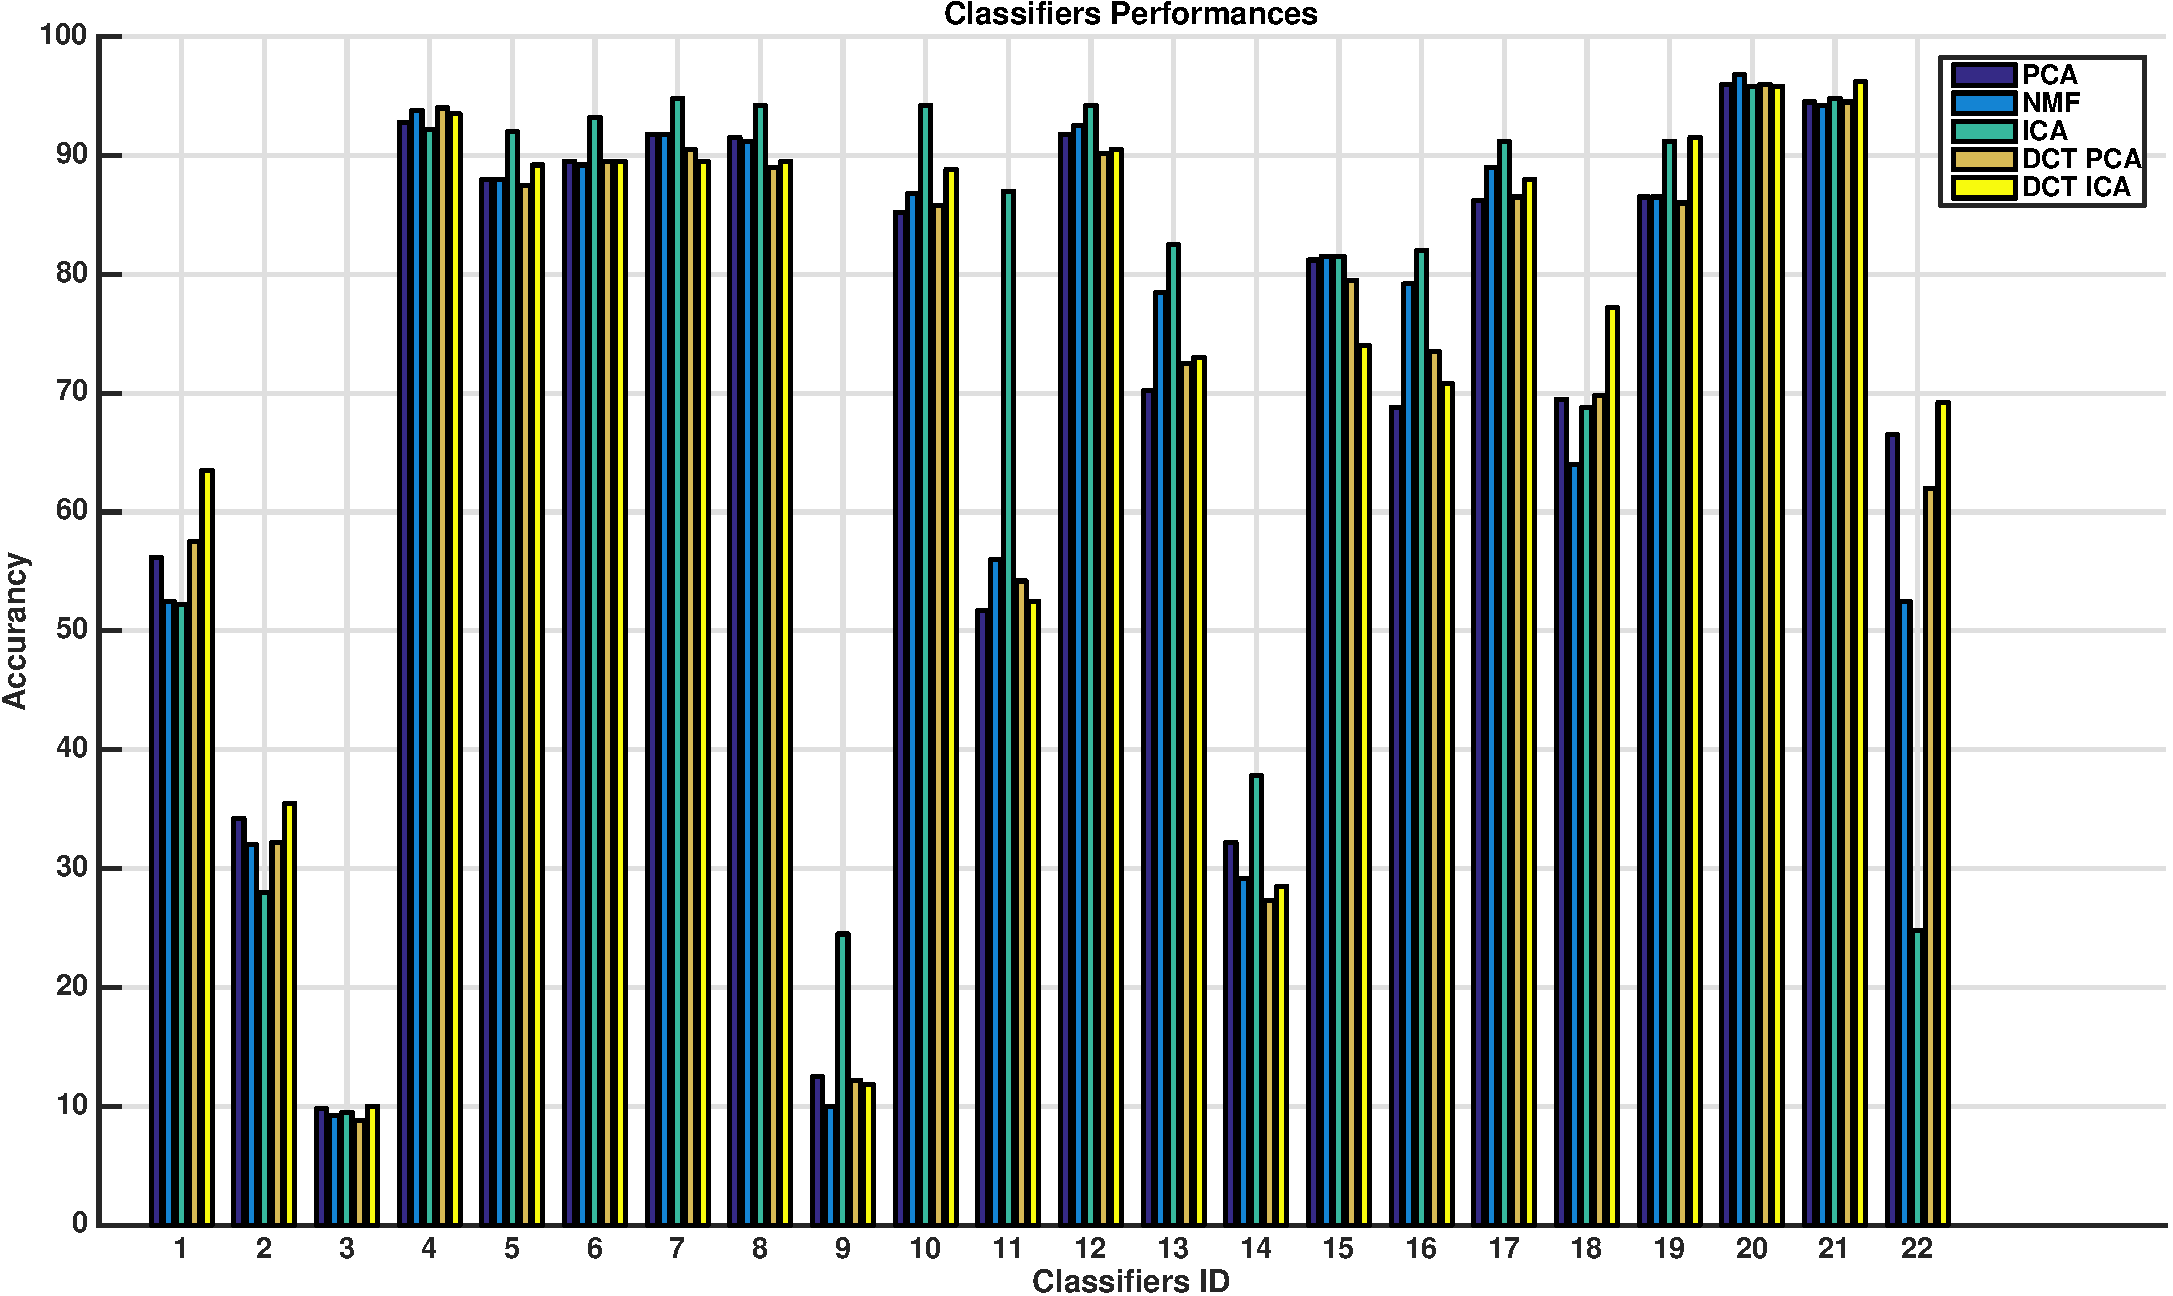
\includegraphics[width=\textwidth]{Img/pni_res} \captionof{figure}{PCA,NMF,ICA结合不同分类机的分类效果\\ ID参见表\ref{table: classifiers}}
	}
	\end{minipage}
	\medskip
	\end{center}
	
\paragraph{结论}
\begin{itemize}
	\item 不提取特征值,而直接压缩图片的方法仍然能很好地和分类机结合
	\item 基于距离的算法,例如KNN算法,就能够很好地识别分类算法可以达到和SVM近似的效果
	\item \textit{Discriminant}方法结合这些特征提取算法的效果较好
	\item 虽然大部分的分类机结合不同的特征提取算法的表现大致相同,但也是存在差异的,如,\textit{Fine Gaussian SVM, Medium Gaussian SVM, Coarse SVM}结合ICA算法的性能就比PCA,NMF好很多
	\item 较高维度下,使用图片压缩算法虽然维数较高,但是可以相比特征提取算法有近似的识别率.
\end{itemize}

\paragraph{分类机对照组} 另外,为了就特征提取这一问题的必要性做出分析,本章节还加入三个参照方法\begin{enumerate} 
	\item 使用\textit{Bicubic}方法压缩的$4 \times 5$图片作为参考. \textit{Bicubic}压缩时使用的公式为
$$ p(x,y) = \Sigma_{i=0}^3\Sigma_{j=0}^3 a_{ij} x_i y_j $$

		\begin{center}
	\begin{minipage}[t]{\linewidth}
	%\label{fig:main}
	\center
	{
	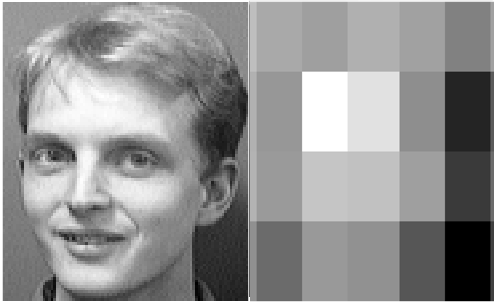
\includegraphics[width=\MyFactor\textwidth]{Img/peo_resize2} \captionof{figure}{\textit{Bicubic}压缩示意,原始大小$112 \times 92$,压缩大小$4 \times 5$}
	}
	\end{minipage}
	\medskip
	\end{center}
	
	\item 使用RCA特征投影算法,RCA是指Random Component Analysis,也就是随机生成基底的方法. RCA使用的基底: 
			\begin{center}
	\begin{minipage}[t]{\linewidth}
	%\label{fig:main}
	\center
	{
	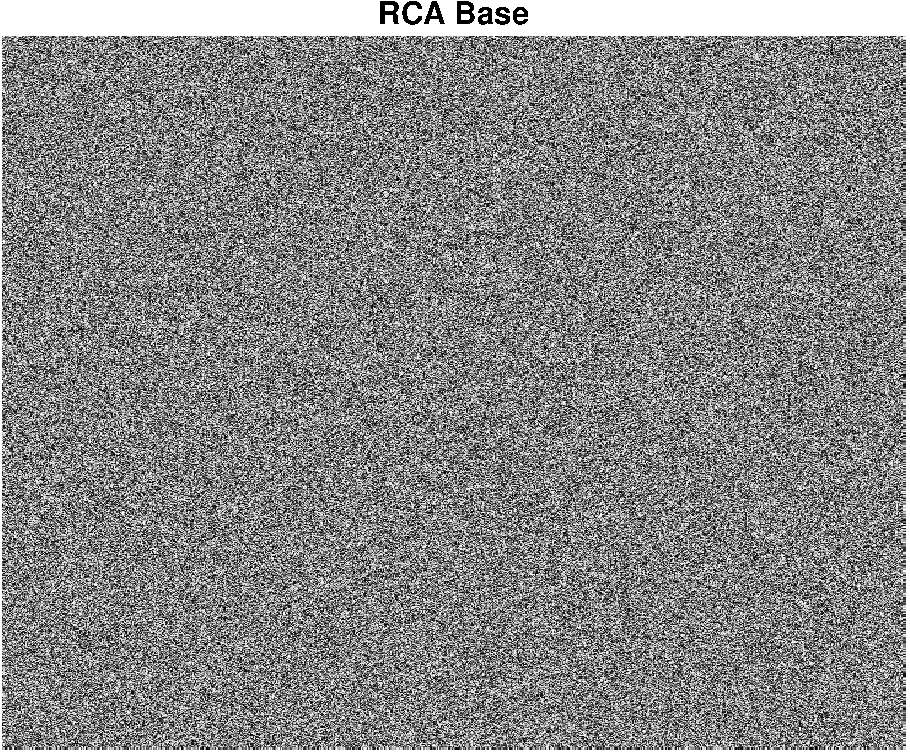
\includegraphics[width=\MyFactor\textwidth]{Img/rca_base} \captionof{figure}{RCA的基底,由于是随机的,64个基底之间的界限不明显}
	}
	\end{minipage}
	\medskip
	\end{center}
	\item 全随机特征值,来测试分类机没有预知标签的信息时的识别性能.

\end{enumerate}

测试结果:

\paragraph{对照组}

	\begin{center}
	\begin{minipage}[t]{\linewidth}
	\center
	{
	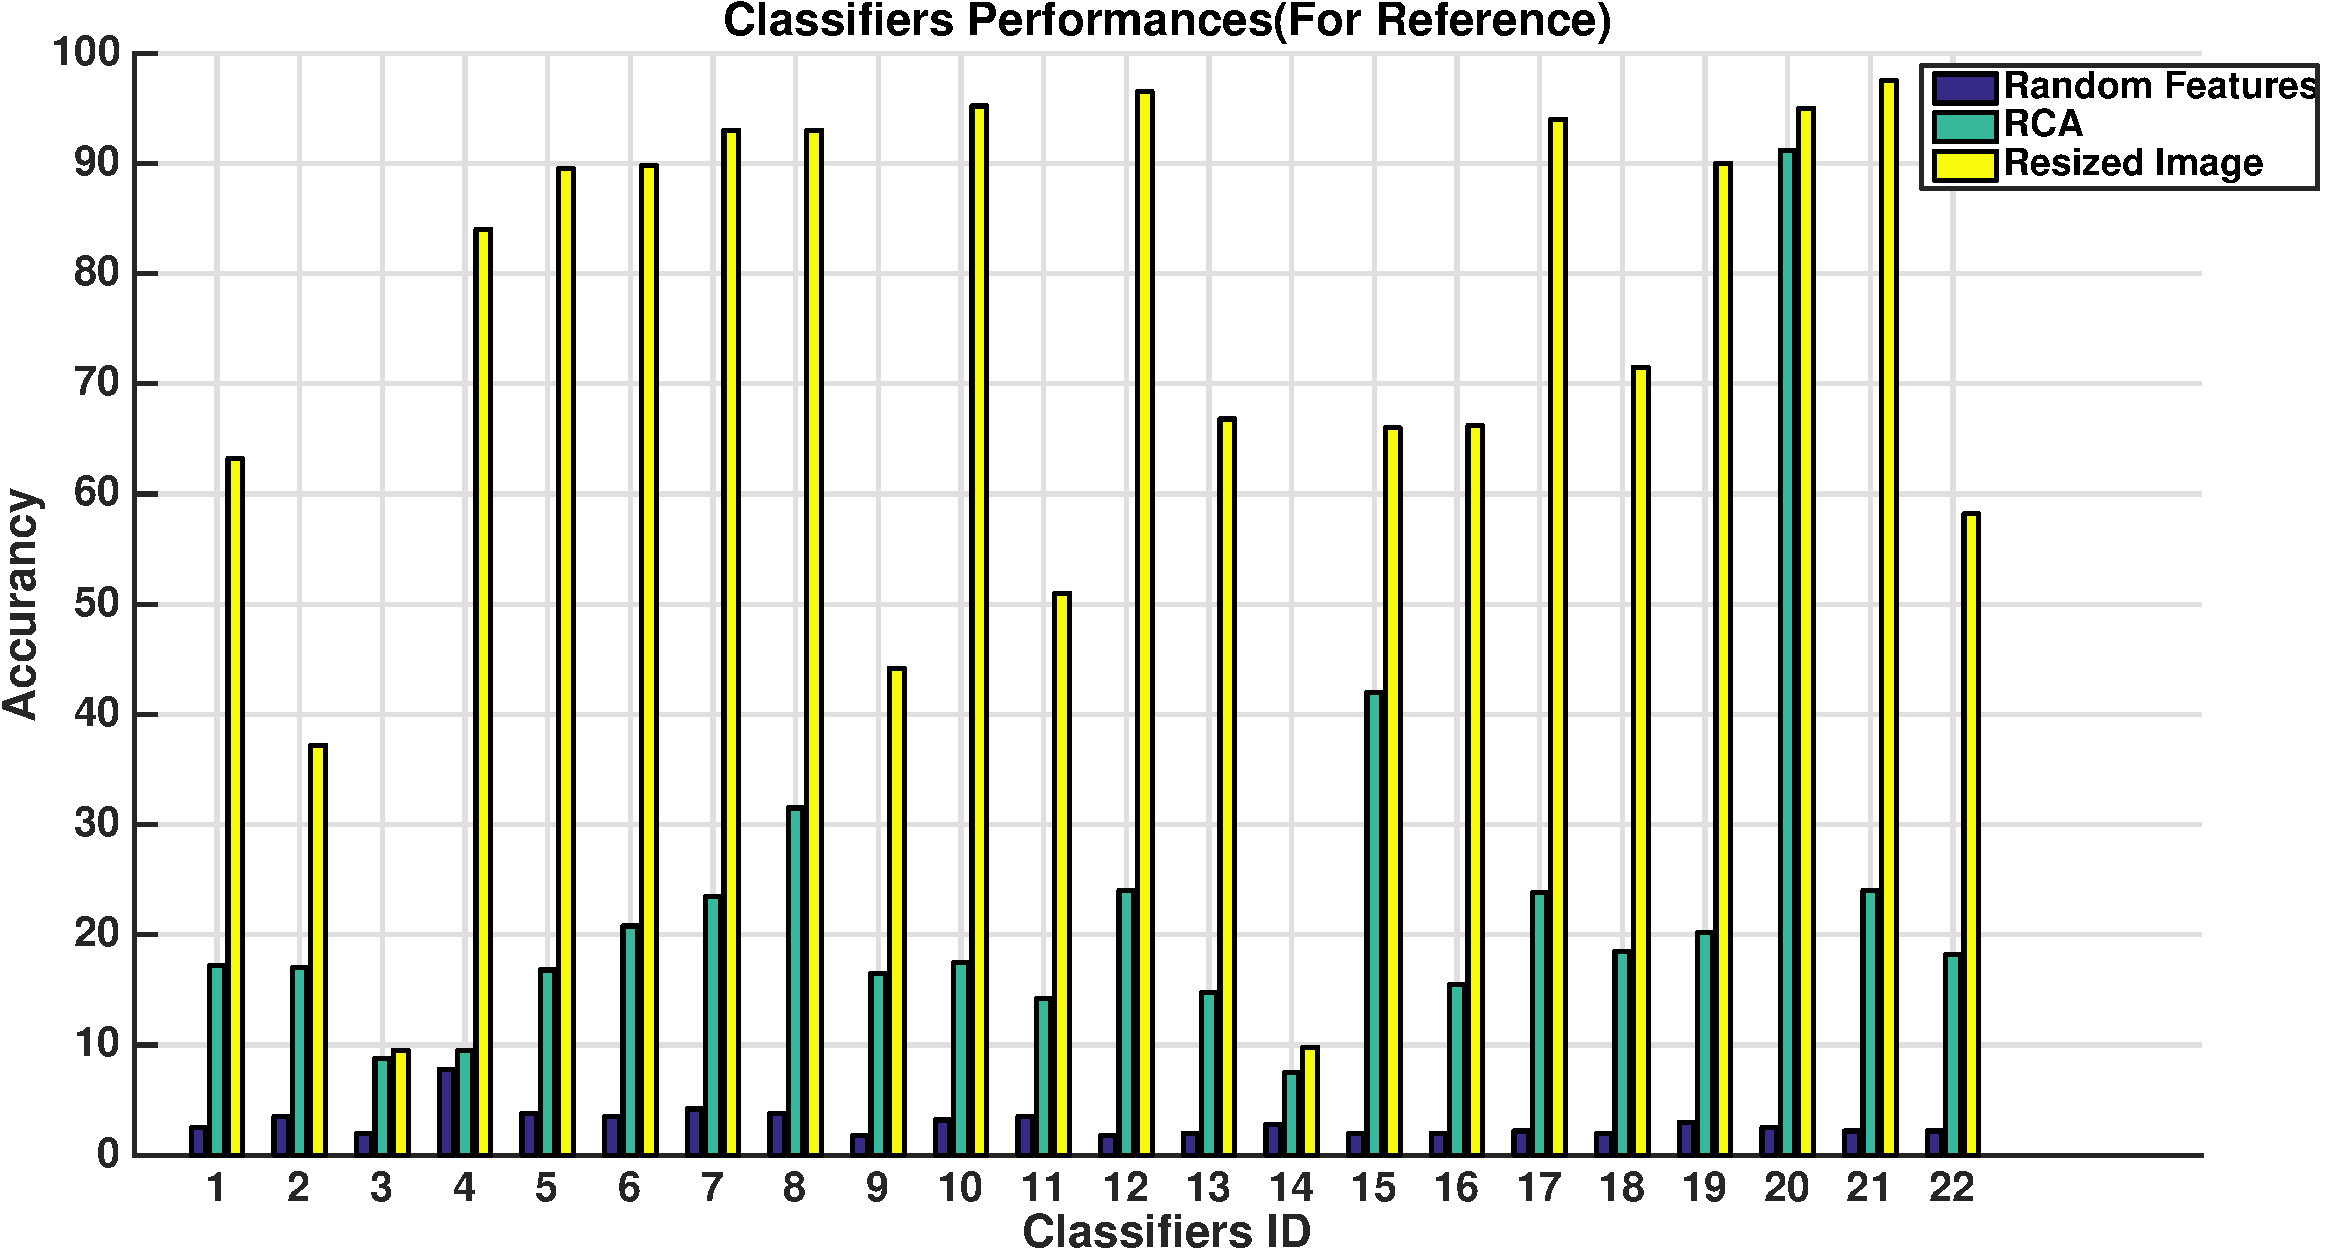
\includegraphics[width=\textwidth]{Img/pni_res_ref.pdf} \captionof{figure}{用来比较的特征算法 \\ ID参见表\ref{table: classifiers}, Resized Image大小为$4 \times 5$}
	}
	\end{minipage}
	\medskip
	\end{center}
\paragraph{结论}
\begin{itemize}
	\item 分类器是没有预知信息的,从随机权值的表现平均仅2.2\%可以看出.
	\item RCA的表现大部分情况并不好,说明了基底的选择与优化是有意义的.
	\item 可以发现,直接对图片采取下采样得到的结果较为优秀,某些情况下还由于特征提取算法.这可能是由于本次输入图片没有背景干扰的原因导致的.一些简单的场景也可以结合一个优化的分类机与下采样算法实现识别.
\end{itemize}
\section{基于局部特征提取算法的相关实验}
\label{sec:comp_local}

\subsection{相关参数}
本部分对\ref{cha:local}中的方法进行测试,这里列举了下列所有测试方法中使用的参数:

\begin{itemize}
	\item SIFT-PCA的基底 \begin{enumerate}
	\item 基底: 120(40个人,每人3张)图片特征空间经过\textit{kmeans}聚类后提取得到的每张图片20个特征空间的全集
	\item 特征向量数: 前20个特征向量,约占50\%的特征值
	\end{enumerate}
	
	\item SIFT和SIFT-PCA的编码方法 \begin{enumerate}
\item 基底: 120(40个人,每人3张)特征点位置的全集
	\item 在固定点描述的方法
	\item 使用\textit{kmeans}聚类	\end{enumerate}
	
	\item SVM参数 \begin{enumerate}
	\item 核函数: 径向基函数 $exp(-gamma*|u-v|^2)$
		\item 径向基函数维度:3
		\item 惩罚函数参数: 0.5
		\item 容错值: 0.001	\end{enumerate}
	
\end{itemize}




\subsection{基底投影的区别}

			\begin{center}
		\begin{minipage}[t]{\linewidth}
		%\label{fig:main}
		\center
		{
		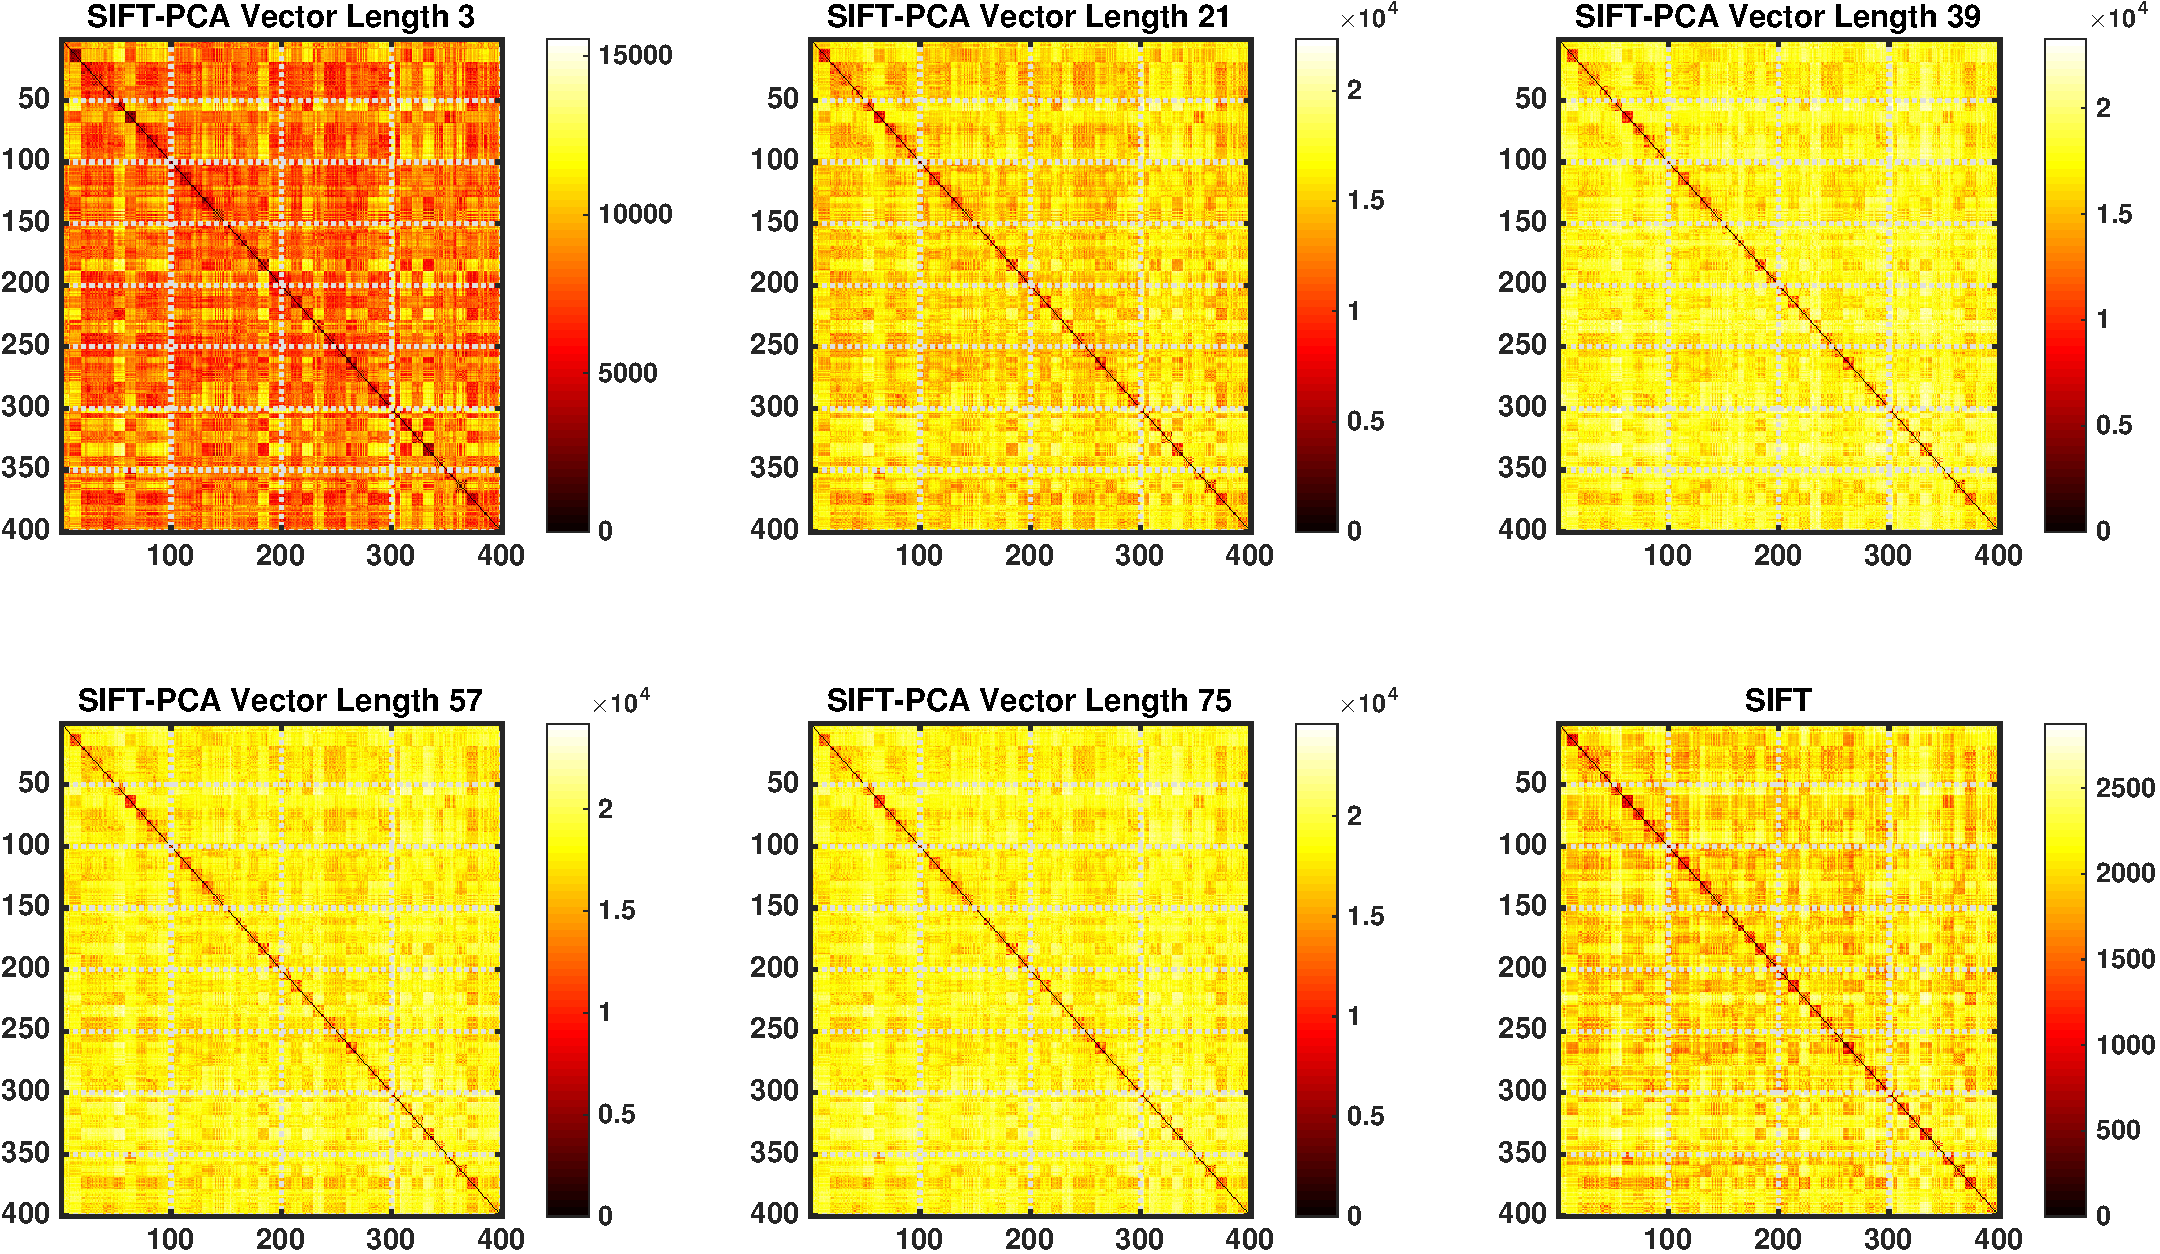
\includegraphics[width=1.1\textwidth]{Img/c3/sift_dis_mat} 
		\captionof{figure}{SIFT及SIFT-PCA的距离矩阵}
		}
		\end{minipage}
		\medskip
		\end{center}
	

\subsection{结合SVM, NKNN的分类实验}
本章采用\textit{Cross Validation Hold Off}的测试方法,测试范围从样本的10\%用来学习到90\%用来学习.来探究不同分类机(SVM, NKNN),SIFT使用不同描述(HoG, SIFT-PCA)时的分类效果.\newline

\paragraph{不同分类机,SIFT使用不同描述时的分类效果}
本节参数,\begin{itemize}
	\item SIFT: 提取3个特征点,并在这些特征点上提取测试图像的特征
	\item 结合NKNN的SIFT-PCA: 提取特征空间,每个特征空间由被提取了20个特征向量
	\item 结合SVM编码的SIFT-PCA: 提取3个特征点,并在这些特征点上提取特征空间,每个特征空间由被提取了20个特征向量
\end{itemize}


下图是分类效果,


		\begin{center}
		\begin{minipage}[t]{\linewidth}
		%\label{fig:main}
		\center
		{
		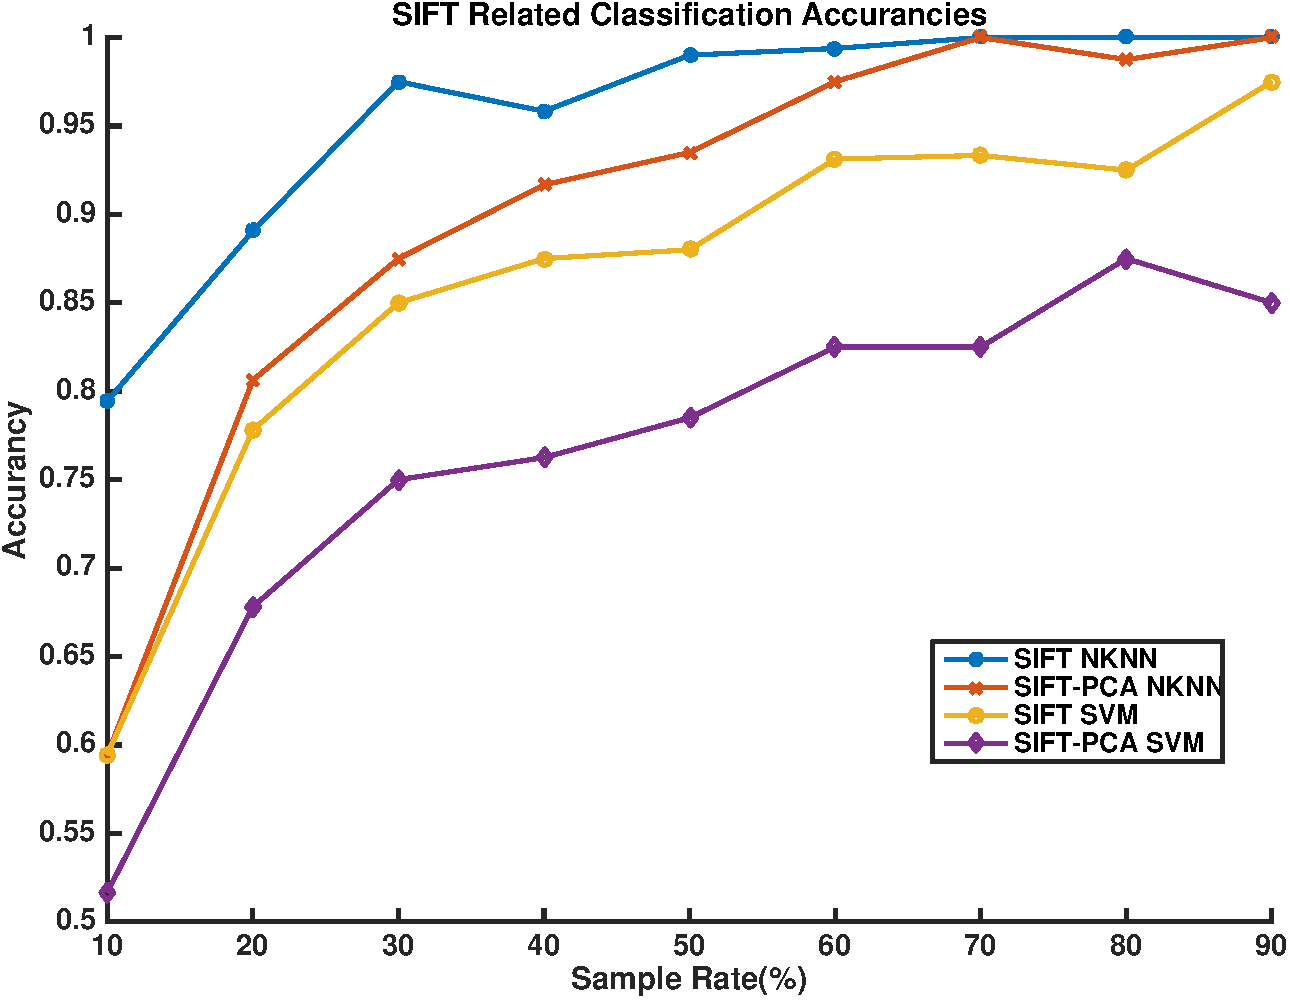
\includegraphics[width=\MyFactor\textwidth]{Img/c3/sift_classification} 
		\captionof{figure}{SIFT-SVM, SIFT-PCA-SVM, SIFT-NKNN, SIFT-PCA-NKNN的比较}
		}
		\end{minipage}
		\medskip
		\end{center}
		
\paragraph{结论:}
\begin{itemize}
	\item 如之前的算法一样,这些算法都是随着样本数的增加而更加精确.
	\item 基于局部的算法有着优良的准确度,如,在学习了50\%的样本后,NKNN算法就能达到近乎95\%的识别率.
	\item NKNN算法的识别率明显优于SVM分类机.这主要是由于NKNN算法无需编码,从而减小了信息损失的缘故.
	\item 实践中,明显感觉基于局部算法的运行效率比基于全局的慢一些,这是由于局部算法的向量长度比较长的缘故.
\end{itemize}

虽然在当前的比较看上去SVM算法比较差,但是这也和编码算法有关,下面部分将就编码算法,样本数和识别率三者之间的关系做进一步讨论.

\paragraph{SIFT, SIFT-PCA的比较}本节参数,
\begin{itemize}
	\item 采用在固定点的编码方法
	\item SIFT-PCA特征向量长度为20
	\item SVM识别方法
\end{itemize}

		\begin{center}
		\begin{minipage}[t]{\linewidth}
		%\label{fig:main}
		\center
		{
		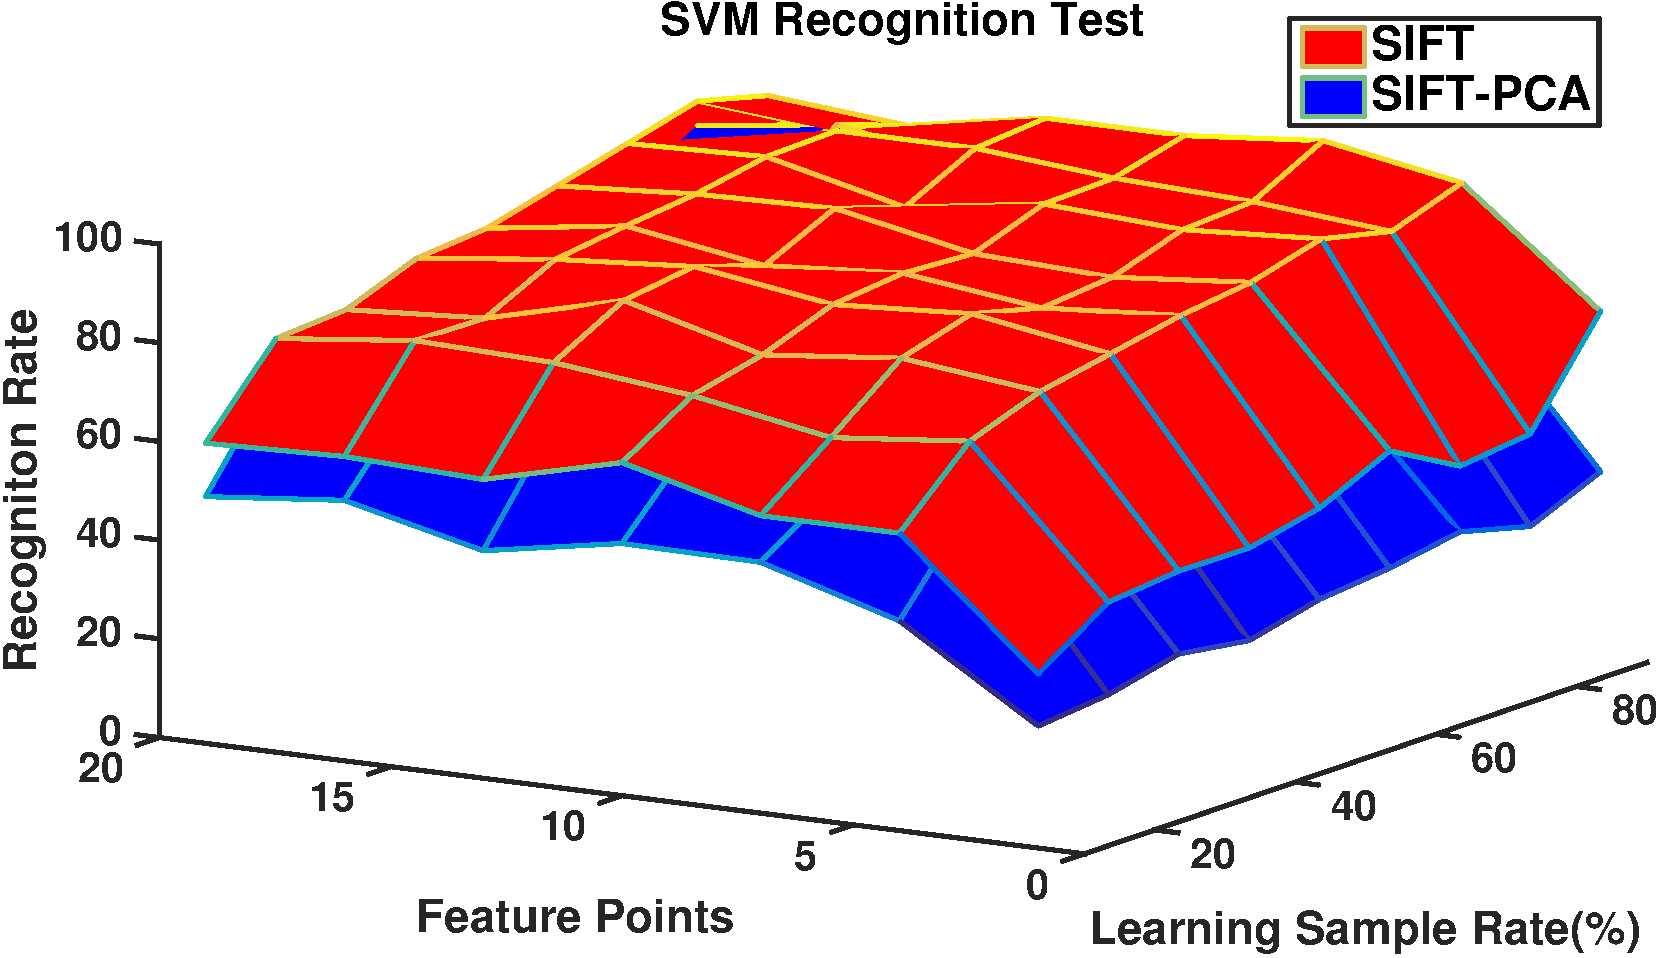
\includegraphics[width=\textwidth]{Img/c3/sift_sift_pca_svm} 
		\captionof{figure}{结合SVM时,SIFT, SIFT-PCA的比较}
		}
		\end{minipage}
		\medskip
		\end{center}
	
\paragraph{结论}
\begin{itemize}
	\item 可见SIFT-PCA的分类效果不如SIFT
	\item 综合来说,SIFT-PCA向量长度为SIFT的$1/5$,而牺牲了10\%左右的识别率
\end{itemize}

\paragraph{SIFT-PCA特征向量变化的影响}
本节参数,
\begin{itemize}
	\item 采用在固定点的编码方法
	\item SVM识别方法
	\item 样本数70\%
\end{itemize}

		\begin{center}
		\begin{minipage}[t]{\linewidth}
		%\label{fig:main}
		\center
		{
		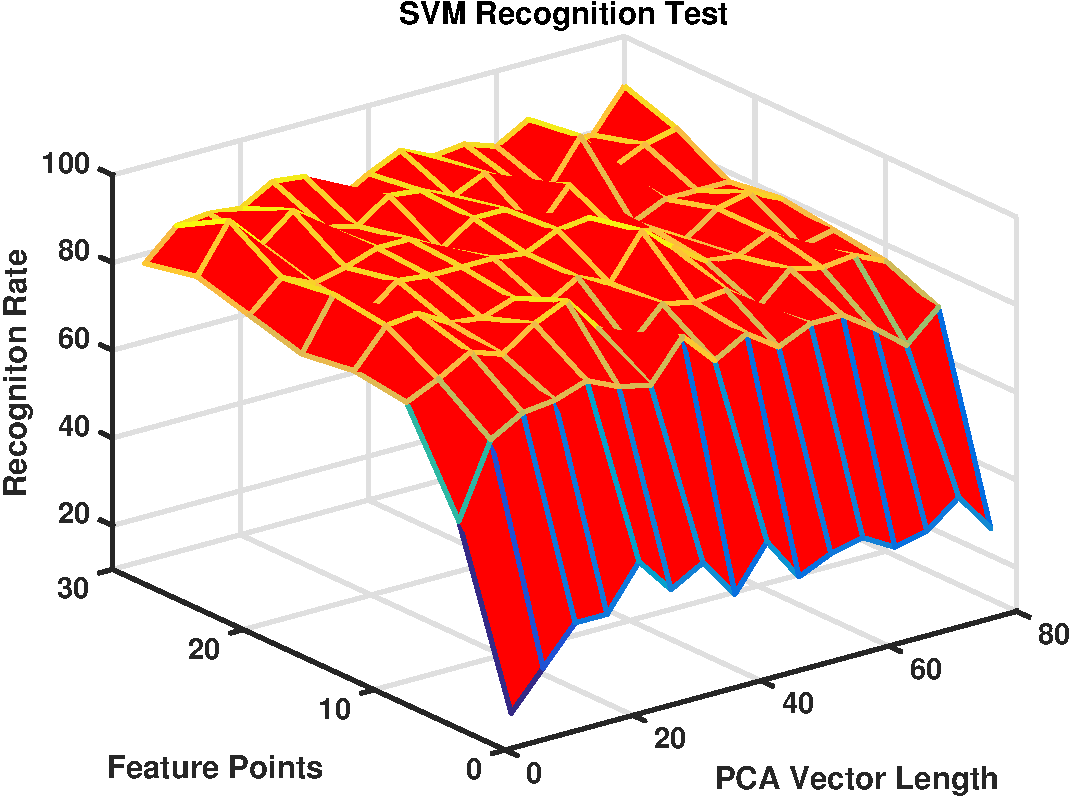
\includegraphics[width=\textwidth]{Img/c3/sift_pca_iter} 
		\captionof{figure}{结合SVM时,SIFT, SIFT-PCA的比较}
		}
		\end{minipage}
		\medskip
		\end{center}

\paragraph{结论}

\begin{itemize}
	\item 可以发现, SIFT-PCA的特征向量长度对识别率的影响并不很大, 所以,在使用SIFT-PCA时,可以使用较高的压缩比
	\item 同时,也发现特征点的数目对识别结果影响较大
\end{itemize}

\subsection{结合多种分类模型的分类实验}
\begin{itemize}
	\item PCA的设置:
		\begin{enumerate}
			\item 使用在kmeans的聚类方法求得特征点位置,共计15个.学习的样本来自120张图片.图片有40个人每人3张得图片组成.
			\item 由于SIFT采用HoG的表示方法,每个特征点为128维向量,综上,每张图片由1920维向量表示.
		\end{enumerate}
	\item SIFT-PCA的设置:
		\begin{enumerate}
			\item 使用在kmeans的聚类方法求得特征点位置,共计15个.学习的样本来自120张图片.图片有40个人每人3张得图片组成.
			\item 使用PCA算法将梯度图片降维到20维.学习的样本来自120张图片.图片有40个人每人3张得图片组成.
			\item 综上,每张图片由300维向量表示.
		\end{enumerate}
\end{itemize}

	\begin{center}
	\begin{minipage}[t]{\linewidth}
	\center
	{
	\captionsetup{justification=centering}
	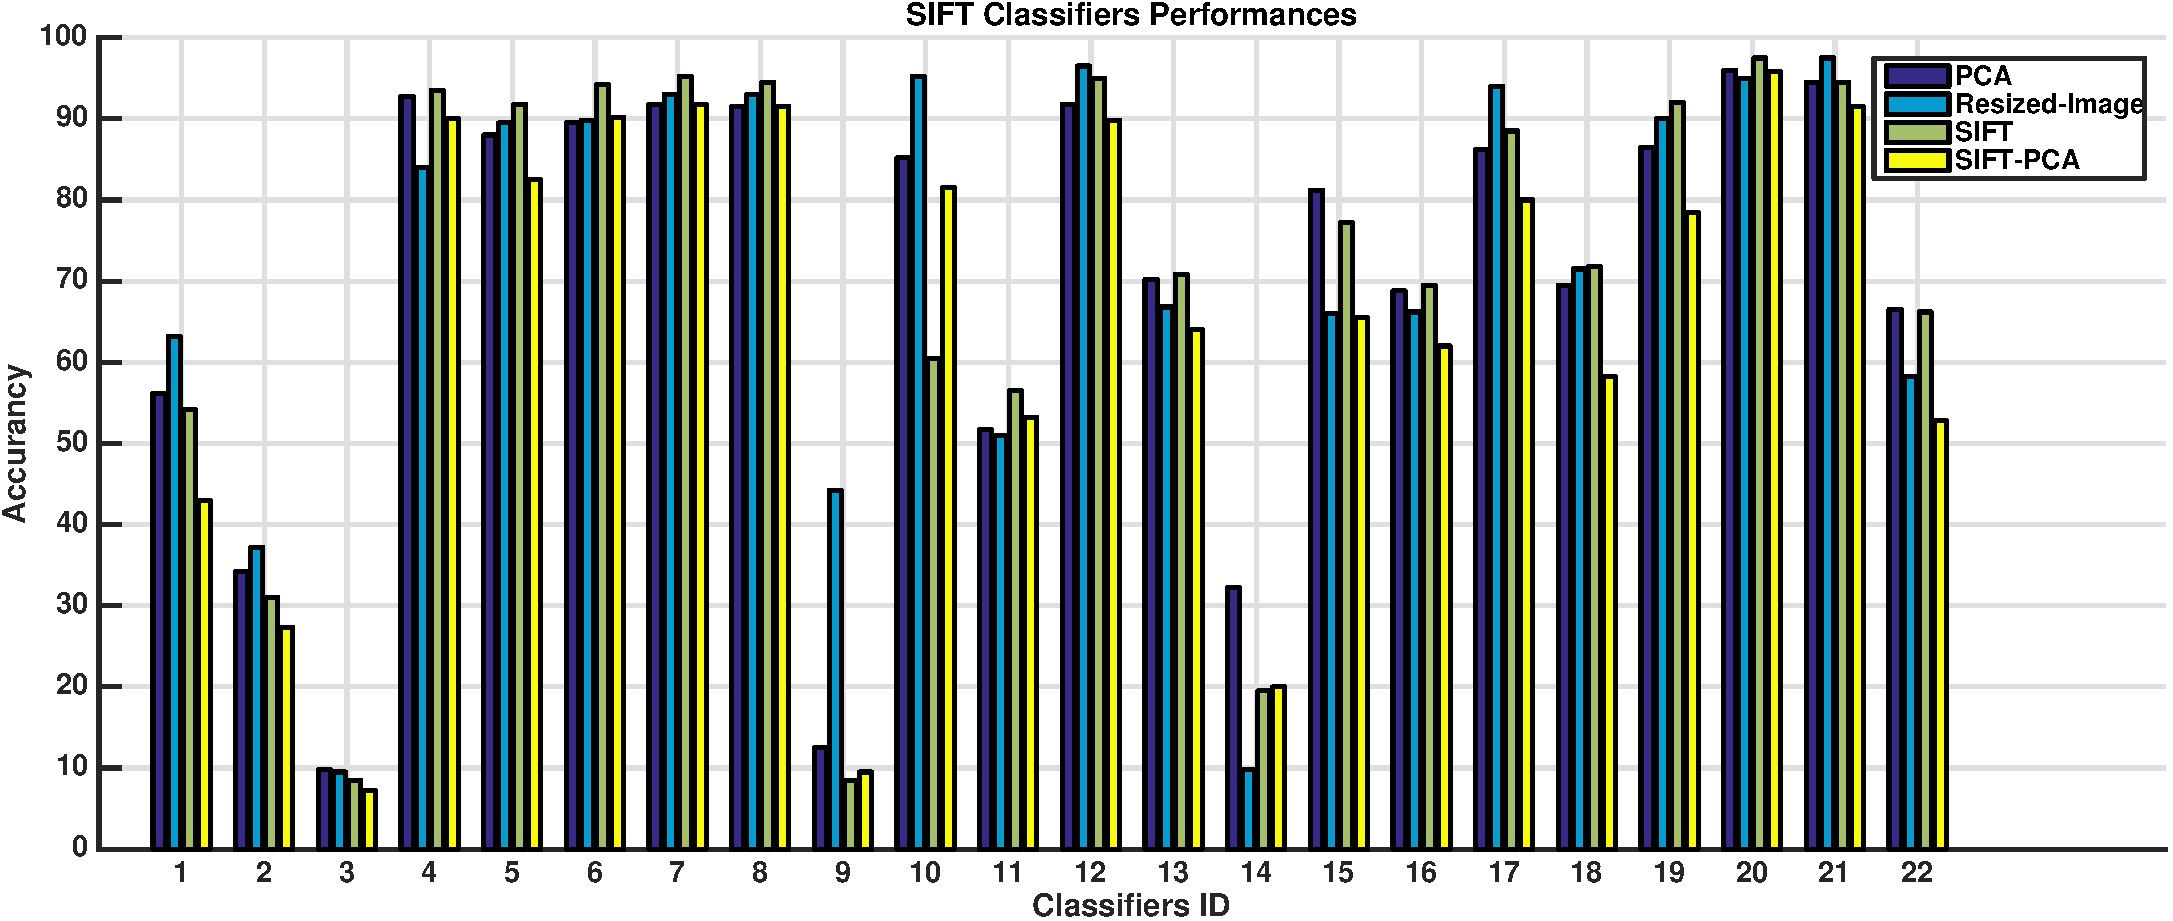
\includegraphics[width=\textwidth]{Img/c3/pni_sift_res} \captionof{figure}{SIFT相关编码后的全局特征提取算法 \\ ID参见表\ref{table: classifiers}, Resized Image大小为$4 \times 5$}
	}
	\end{minipage}
	\medskip
	\end{center}
\paragraph{结论}
\begin{itemize}
	\item 和之前大多数情况一样,该配置下大部分情况下SIFT表现优于SIFT-PCA.但是差别并不很大,并且SIFT-PCA长度大大短于SIFT.
	\item 在编码方式后,由于信息丢失,SIFT结合普通分类机的表现并没有优势.说明好的特征提取算法也需要与对应的分类机结合.
\end{itemize}

\section{综合比较:不同尺度下的性能}

下面将就各种特征提取算法在不同尺度下的性能做出比较. \newline

由于本毕业设计中涉及了较多的算法,所以全部加入比较会使结果非常冗长.通过对之前两小节的比较,笔者选择出了一些有代表性的算法,在此结合图片维度的变化来一并做出比较.这些算法及其参数:
\begin{enumerate}
	\item PCA结合SVM分类机
	\item ICA结合SVM分类机
	\item SIFT结合编码算法后结合SVM分类机
	\item SIFT\_PCA结合NKNN算法
\end{enumerate}
参数和之前一样,分别是:
\begin{
	\item SIFT-PCA的基底 \begin{enumerate}
	\item 基底: 120(40个人,每人3张)图片特征空间经过\textit{kmeans}聚类后提取得到的每张图片20个特征空间的全集
	\item 特征向量数: 前20个特征向量,约占50\%的特征值
	\end{enumerate}
	\item SIFT和SIFT-PCA的编码方法 \begin{enumerate}

%\section{F-Score}
%以上章节仅就\textit{识别率}这一指标来评价,实际上,这是不全面的,因为没有考虑\textit{False Positive}和\textit{True Negative}的矛盾问题,具体来说,
%\begin{itemize}
%	\item 在搜索人脸的过程,人们通常希望系统能提出更多的候选图片,这就需要降低系统阈值,使得更多的答案能被接受.这时候,\textit{Positive}的比例就希望大一些,但这提升了\textit{False Positive}降低了\textit{True Negative}.
%	\item 在较为精密的系统中,如使用人脸作为密码进行支付,人们通常希望提高系统阈值.\textit{Negative}的比例就希望大一些,但这降低了\textit{False Positive}提升了\textit{True Negative}.
%\end{itemize} 
%下面就本文模型中较好结果计算了它的F-Score.
%

\section{结论与展望}

近半年的毕业设计终于告一段落了,笔者在其中学到了不少知识,如降维算法,模型评价等知识.但是,受限于个人能力和时间投入的原因,有很多地方只得匆忙完成,不能再深入讨论下去了,本部分将可以深入探究的地方罗列一下,期望日后能得以机会加以完善.

\paragraph{全局识别的第二种架构}
本文所有的全局识别算法都是建立在以人脸图像为基本单元的基础上,由于人脸图像样本数目远小于像素的数目,这样做比较快.但是,也不可否认,存在第二种方法.在\ref{sec:arch2}中列出了以像素为基本单元的方法.目前由于运算时间的问题没能继续下去.

\paragraph{NMF算法的迭代方法研究}
本文所用的NMF迭代算法是比较早的算法,根据\cite{lin2007projected}. 本文所用的NMF算法是存在一定问题的,作者希望就NMF这一算法深入研究.

\paragraph{ICA算法应用于图片压缩}
作者在研究论文时,发现了将图片切割并使用分块的PCA或ICA来实现图像压缩的算法.以图\ref{fig:ica_base}为例,ICA算法有很强的稀疏性,因此适合以保留主要参数的方法进行图片压缩.ICA图像压缩由于不是在频谱上压缩,因此有保留图像细节的优点.

\paragraph{章节\ref{sec:pni_recon}的应用}
实际上\ref{sec:pni_recon}中MSE的差别可以被加以利用来识别场景的.可以看到,人脸压缩并恢复后的图像的与原始图像的差别小于非人脸压缩并恢复后的图像,这可以从这个角度识别人脸.

\paragraph{SIFT算法的编码方法}
本文实现的SIFT编码方法比较粗略,实际上还存在更多更加优秀的算法,受限于时间作者没能一一实现.

\paragraph{Gabor算子}
本文的局部特征提取算法只实现了SIFT算法,实际还有\textit{Gabor}等算法,作者希望有机会时把这部分内容也加进去.

\paragraph{KD树进行人脸搜索}
实际上,本项目还实现了基于距离的人脸搜索过程,但是,很遗憾的,仅仅基于距离很难搜索到相近的人.因此该部分并没有产生较好的结果,作者希望可以加以模糊逻辑等方法来优化这个过程.同时,作者指出这个方法的优越性,距离搜索可以通过KD树来完成,性能非常好,可以分布计算,非常构建人脸数据库,在大量人群中快速搜索.

\paragraph{算法比较的其他指标}
以上章节仅就\textit{识别率}这一指标来评价,实际上,这是不全面的,因为没有考虑\textit{False Positive}和\textit{True Negative}的矛盾问题.笔者拟结合\textit{F-Scrore}这个参数来和\textit{识别率}一起表征算法的性能.
